% !TEX encoding = UTF-8
% !TEX TS-program = pdflatex
% !TEX root = ../Tesi.tex
% !TEX spellcheck = en-EN

%************************************************
\chapter{Validation}
\label{cap:validation}
%************************************************

\section{DEM Simulations}
\label{sec:simulations}

For sinter fine, 546 shear cell and 81 static $AoR$ simulations 
\wrong{write down all the simulations performed at the end.}
were run with
the parameter combinations described in Table
\ref{tab:10DEMVariableinputvalues}.
The computational time amounted to 1 hour with 32 AMD cores for a benchmark
shear-cell simulation and to 9 hours for a benchmark $AoR$ simulation, both with
50,000 particles.
Simulations with larger $dCylDp$ required more time (e.g., about 12 hours for
the shear cell with 400,000 particles ). \\

\begin{table}[h]
\centering
\begin{tabular}{ccccc}
\hline
    \acs{mus} & \acs{mur} & \acs{CoR} & \acs{rhop} & \acs{dCylDp} \\
    	$[-]$  & $[-]$   & $[-]$   & $[kg/m3]$ & $[-]$ \\
    \hline
    0.4 / 0.6 / 0.8 & 0.4 / 0.6 / 0.8 & 0.5 / 0.7 / 0.9 & 2500 / 3000 / 3500 & 20 / 36 / 38 / 40 \\

\hline
\end{tabular}
\caption[DEM variable input values]{DEM variable input values for training the
Neural Networks}
\label{tab:10DEMVariableinputvalues}
\end{table}.

\section{ANN model development}
\label{sec:annmodeldev}

\begin{table}[htbp]
  \centering

    \begin{tabular}{lccc}
    \hline
          & Bayesian & Gaussian & ANN \\
          \hline
    Coefficient of determination ($R^2$) & 0.86  & 0.843 & 0.959 \\
    Root mean squared error & 0.057 & 0.061 & 0.031 \\
    Mean absolute error & 0.042 & 0.038 & 0.025 \\
    Mean squared error & 0.003 & 0.004 & 0.001 \\
    \hline
    \end{tabular}%
      \caption{Regression methods quantitative comparison.}
  \label{tab:14regressionvalues}%
\end{table}%

First, we determined the regression of the bulk behaviour parameters, for
instance the $\mu_{psh}$, 
with a Bayesian linear prediction (Fig.
\ref{fig:069sctbayesianlinearregressor}) and a Gaussian nonlinear prediction
(Fig.  \ref{fig:070sctgaussiannonlinearregressor}). 
Later we obtained Fig.
\ref{fig:071annnonlinearregressor}, where the corresponding plot for the $ANN$ with the maximum $R^2$ is shown. 
Each circle represents one of the 546 simulations.
\wrong{write down all the simulations performed at the end.}
Table \ref{tab:14regressionvalues} shows a quantitative comparison between the
three methods. 
In fact, 
we achieved a $R^2 = 0.96$ for an $ANN$ with fifteen neurons,
a consistent agreement between the 
$DEM$ and the $ANN$ values, which demonstrates the accurate predictive power of
the $ANN$.\\ 
Increasing the number of neurons did not improve the $R^2$; it even started to
oscillate with higher numbers of neurons.
We subsequently obtained the optimal number of neurons for all $ANNs$.
Further, we processed the random combinations (Table
\ref{tab:10DEMVariableinputvalues}) with the $ANN$.
The $ANN$ evaluation was significantly faster than the $DEM$ simulations. The
individuation of the numerical bulk behaviours for all the $DEM$ combinations
did not take more than a few seconds on a single core.
%************************************************
\begin{figure}[!h] 
\centering 
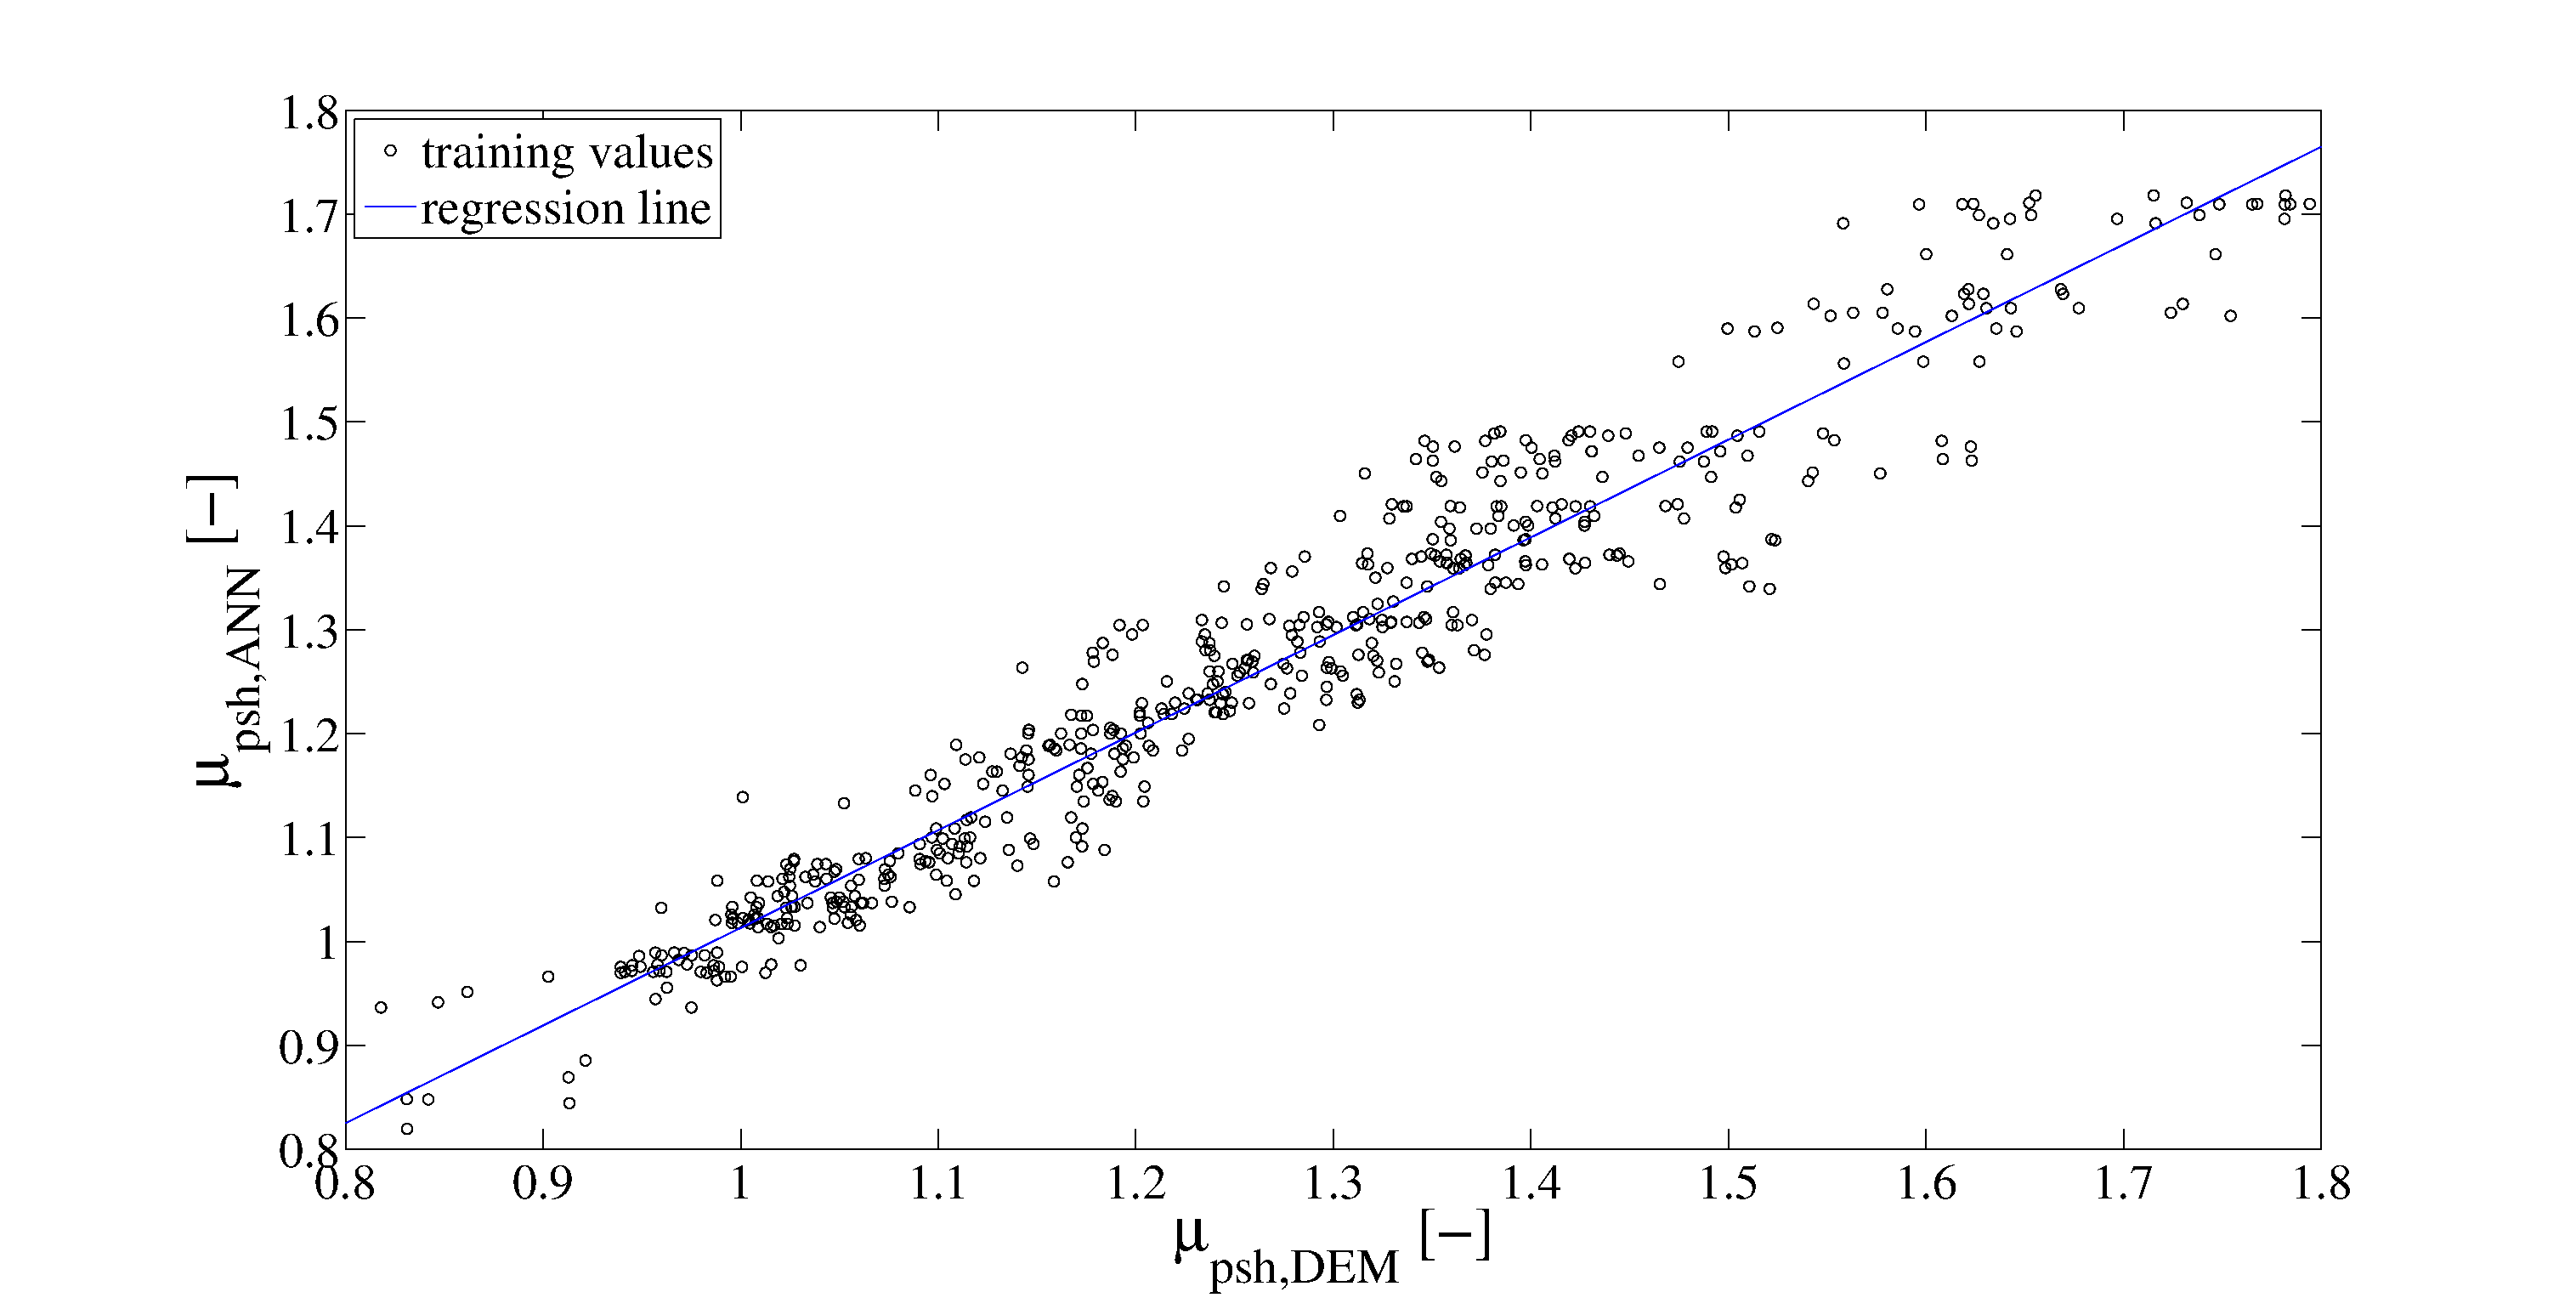
\includegraphics[width=.80\columnwidth]{images/022regression.eps}
%[width=.96\textwidth]
\caption[Comparison between prediction of the trained ANN and full DEM
simulation]{Comparison between prediction of the trained Artificial Neural
Network (\acs{ANN}) and 546 
\wrong{write down all the simulations performed at the end.}
full DEM simulations of the coefficient of pre-shear
(\acs{mupsh}).}
\label{fig:022regression} 
\end{figure}
\improvement{Decide how many regression images are necessary.}

	  \ref{fig:069sctbayesianlinearregressor}\\

	  \ref{fig:071annnonlinearregressor}\\

	  \ref{fig:072aorbayesianlinearregression}\\

	  \ref{fig:073aorgaussiannonlinearregression}\\

	  \ref{fig:074aorannnonlinearegression}\\
  \ref{fig:077regressions}\\
\begin{figure}[htbp]
  %\null\hfill
  \subfloat[SCT Bayesian linear regressor.]{
	  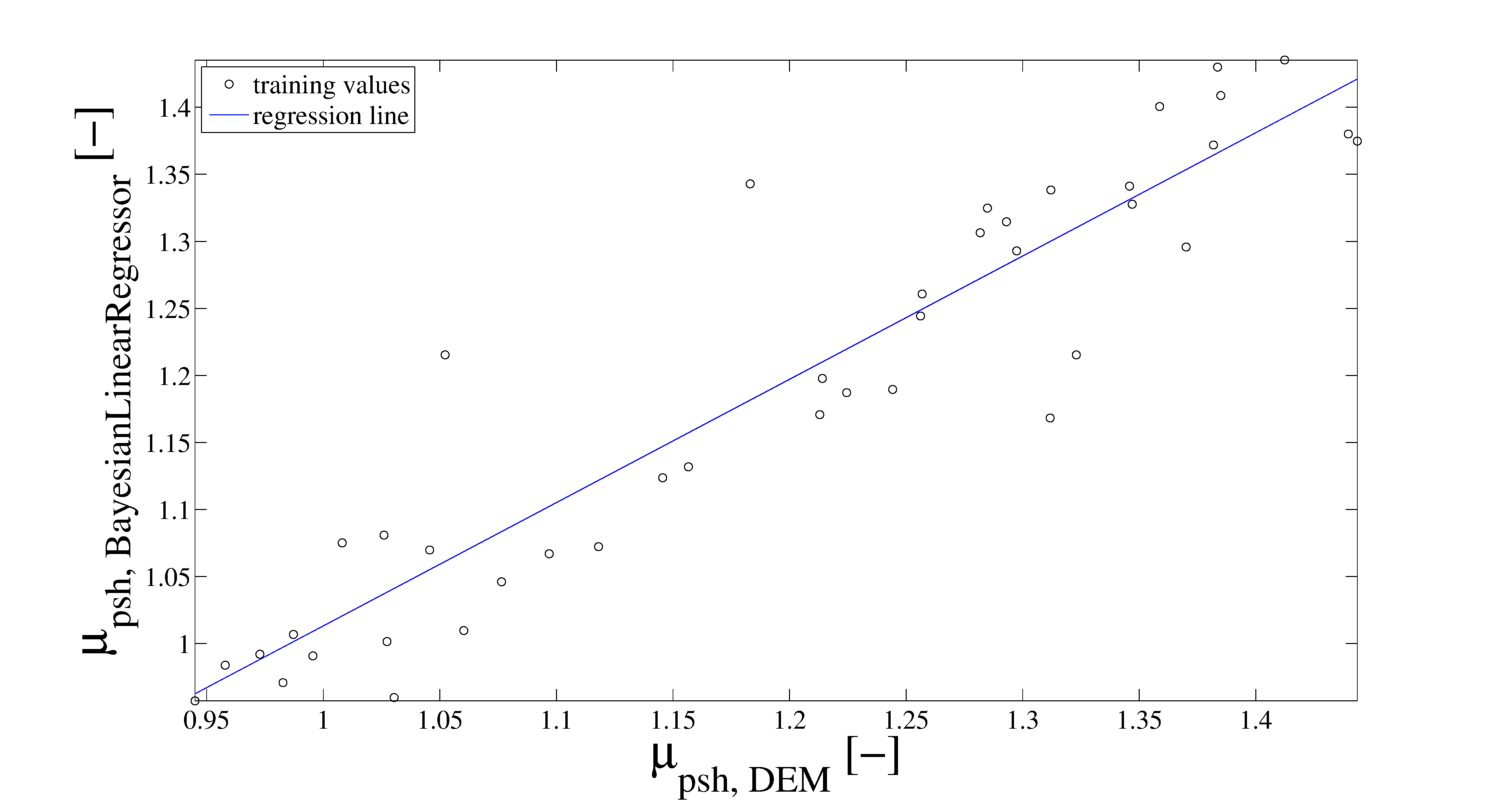
\includegraphics[width=.48\columnwidth]{images/069sctbayesianlinearregressor}
	  \label{fig:069sctbayesianlinearregressor}
  }
  \quad
    \subfloat[SCT Gaussian non linear regressor.]{
	  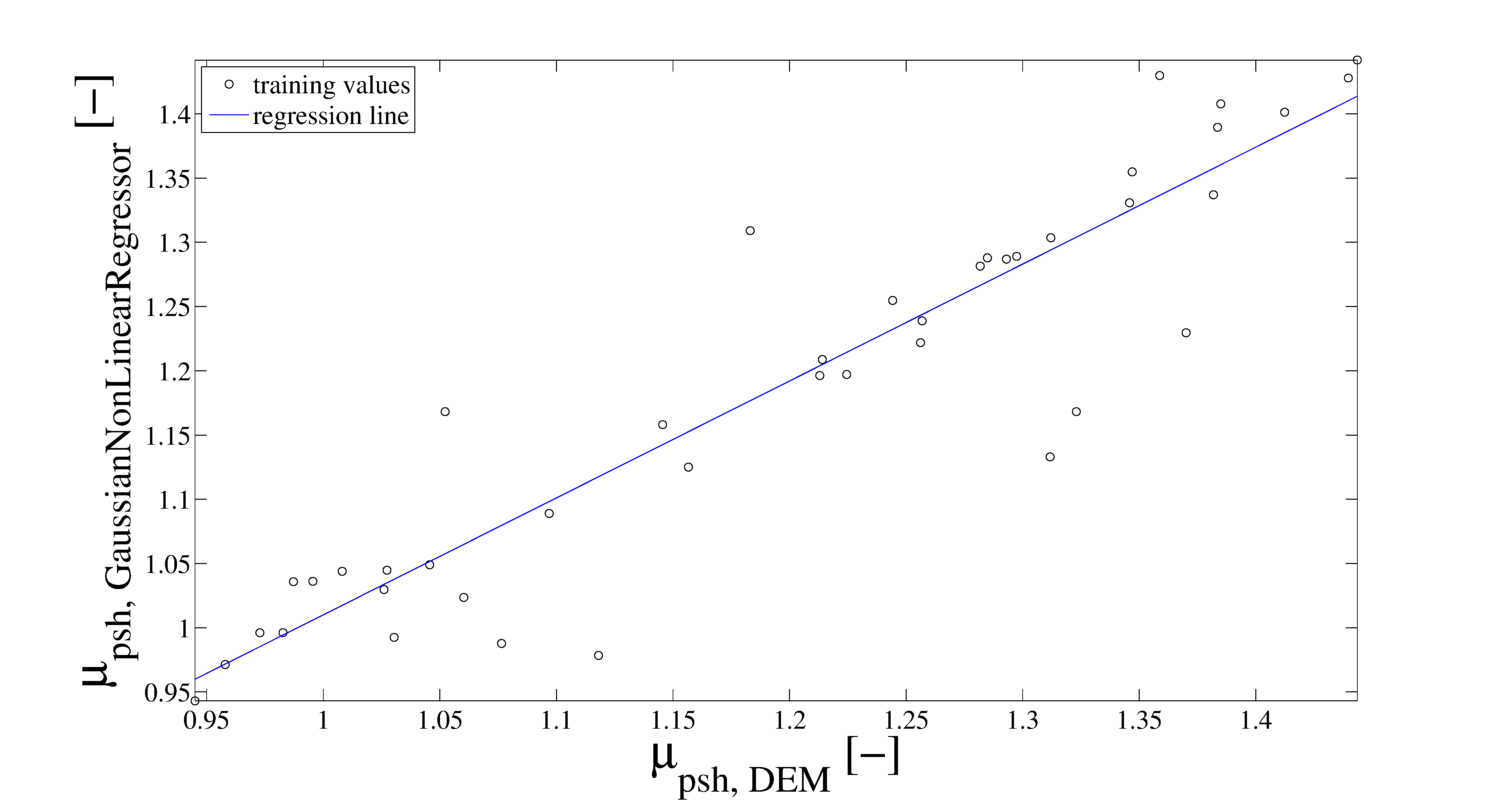
\includegraphics[width=.48\columnwidth]{images/070sctgaussiannonlinearregressor}
	  \label{fig:070sctgaussiannonlinearregressor}
  }
  \\
 % \hfill
  \subfloat[SCT ANN non linear regression.]{
	  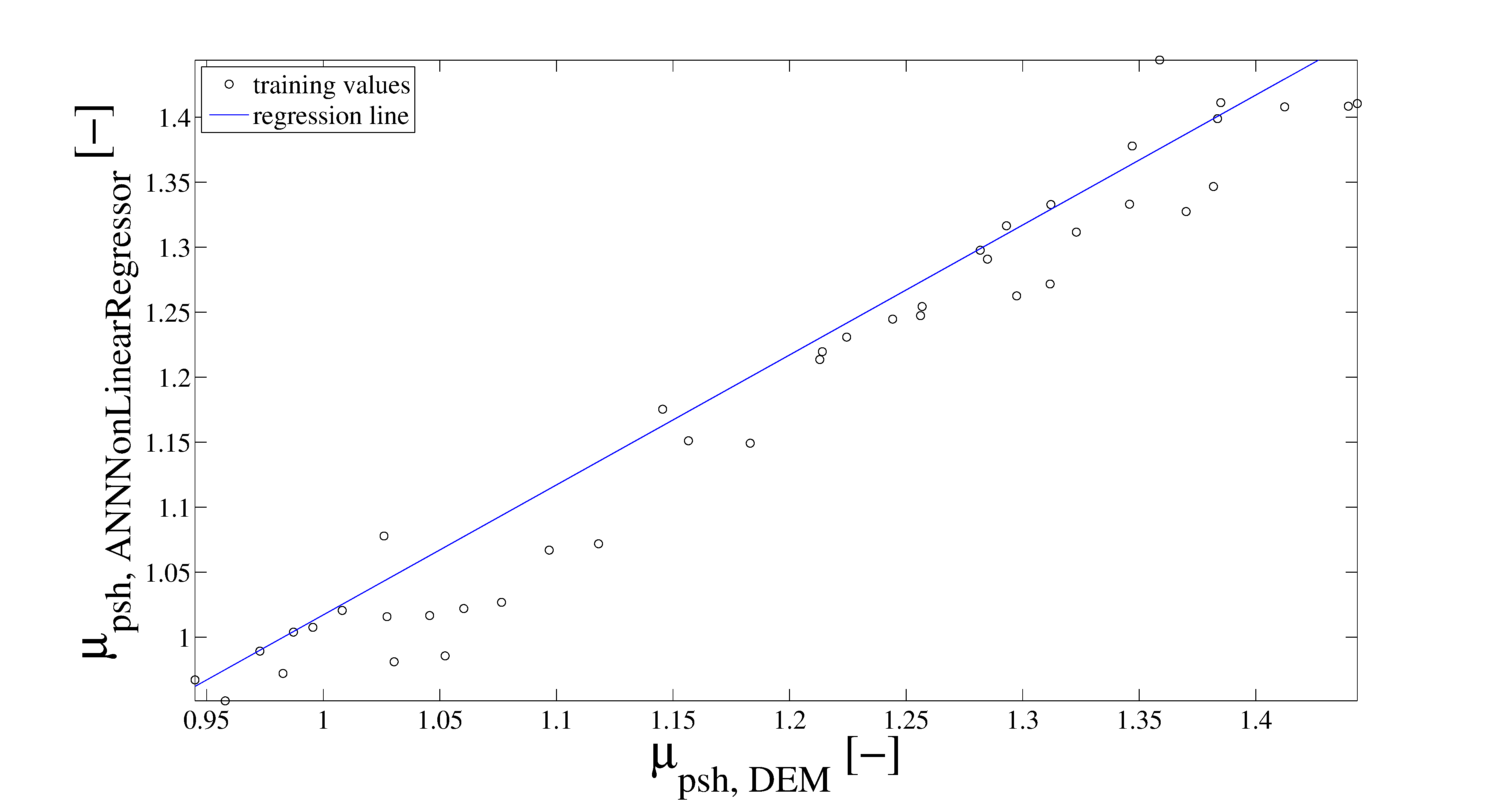
\includegraphics[width=.48\columnwidth]{images/071annnonlinearregressor}
	  \label{fig:071annnonlinearregressor}
  }
  \quad
    \subfloat[AoR Bayesian linear regressor.]{
	  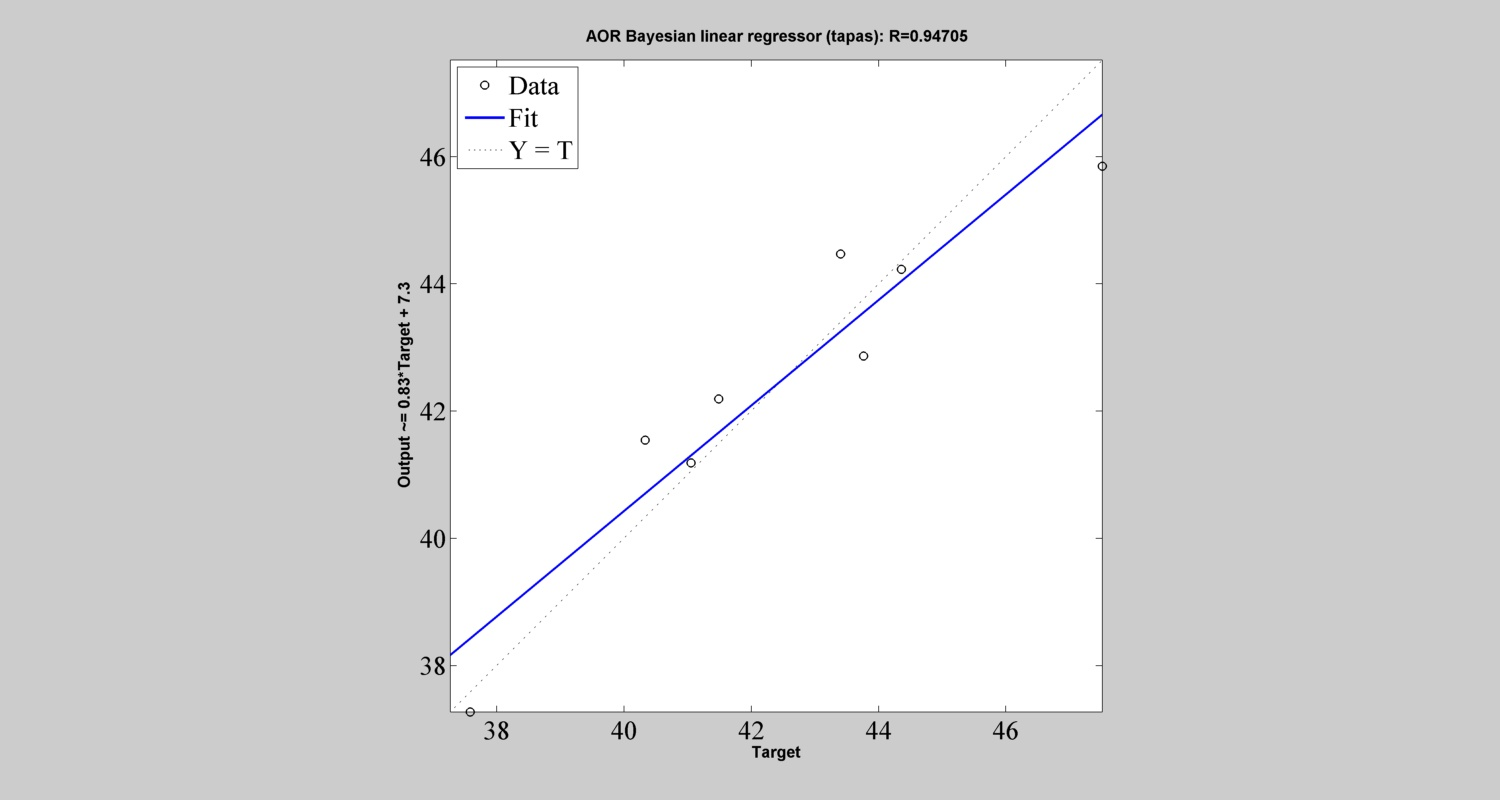
\includegraphics[width=.48\columnwidth]{images/072aorbayesianlinearregression}
	  \label{fig:072aorbayesianlinearregression}  }
  \\
    \subfloat[AoR Gaussian non linear regressor.]{
	  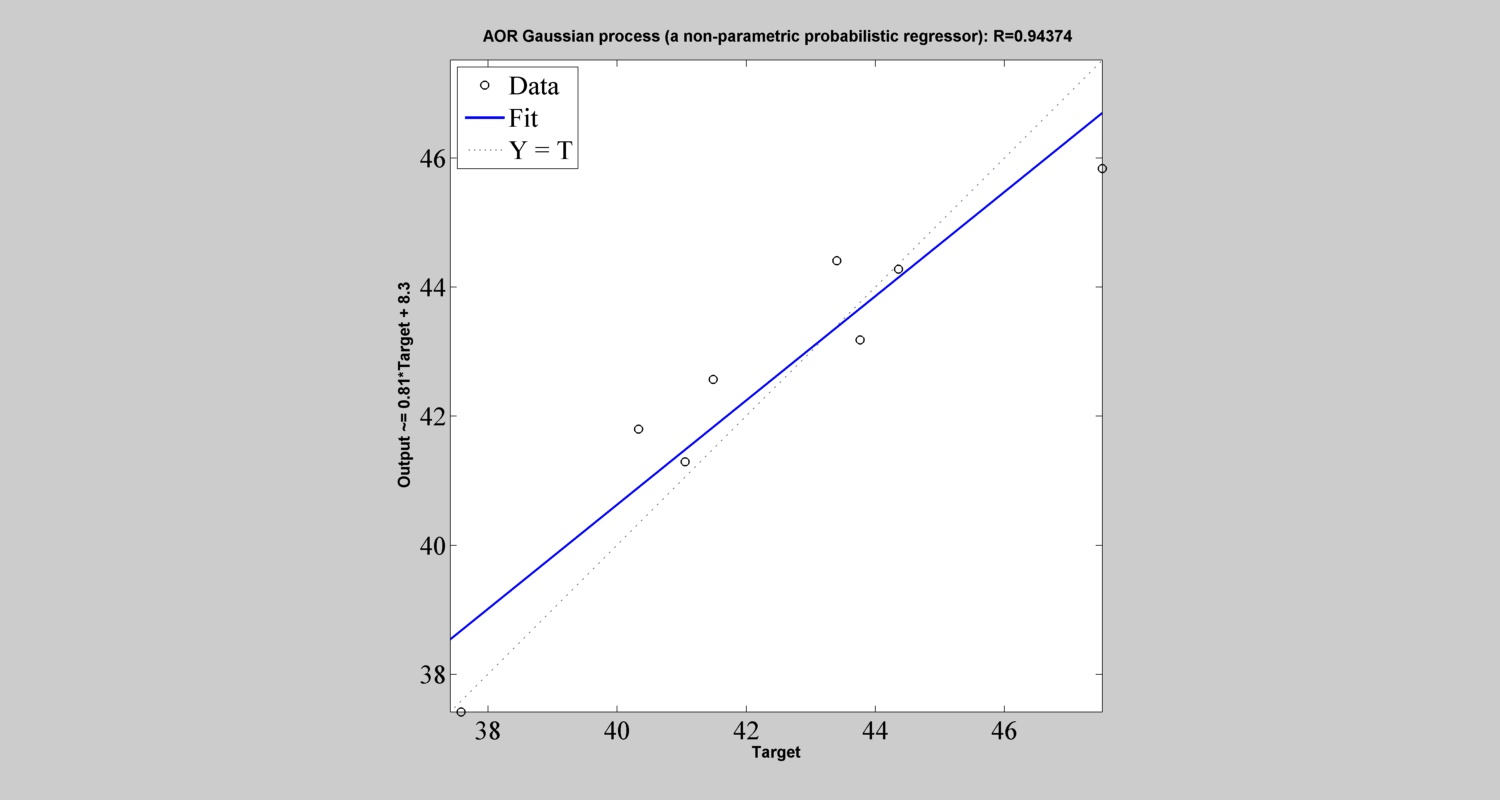
\includegraphics[width=.48\columnwidth]{images/073aorgaussiannonlinearregression}
	  \label{fig:073aorgaussiannonlinearregression}
  }
  \quad
 % \hfill
  \subfloat[AoR ANN non linear regression.]{
	  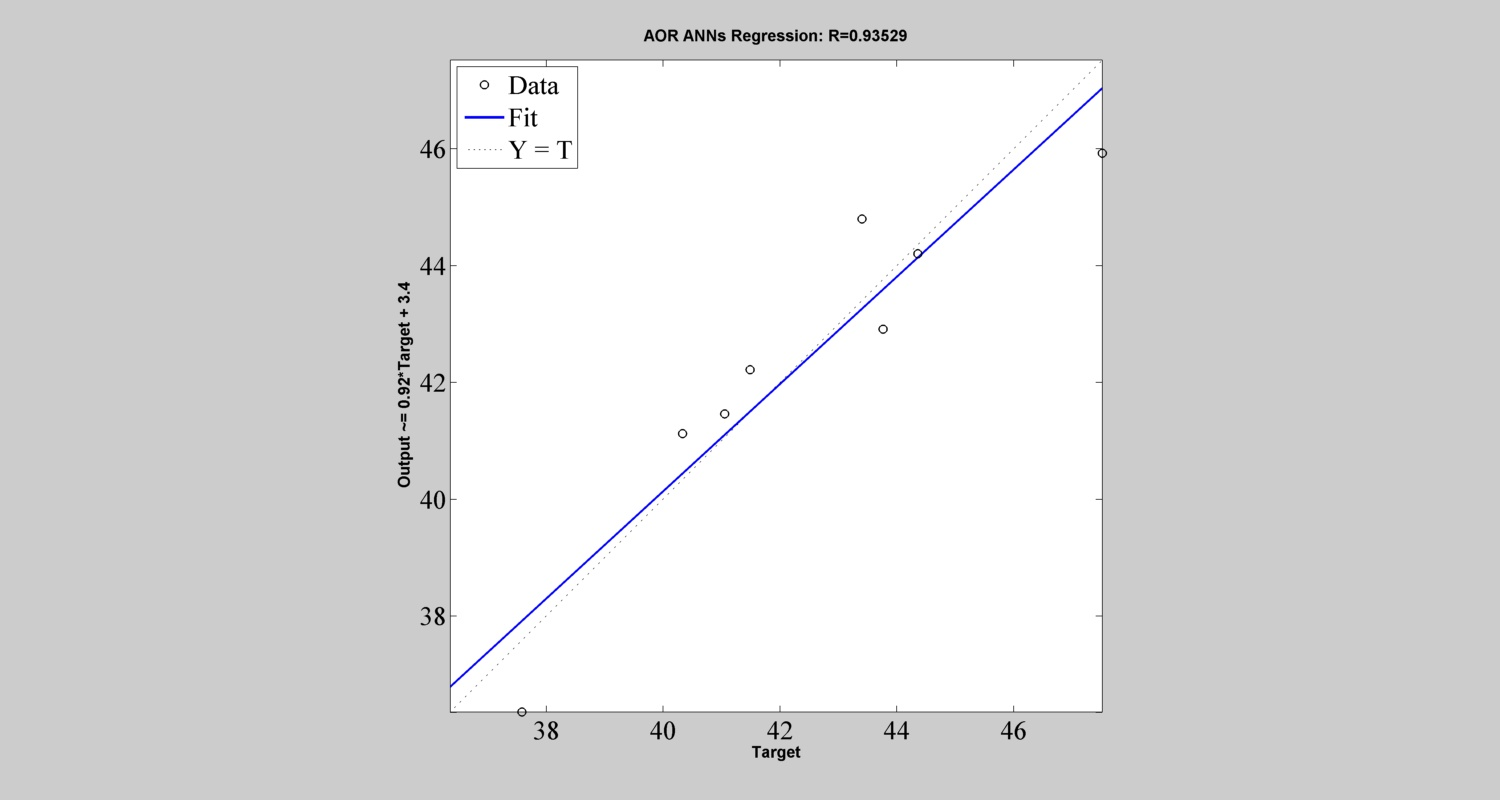
\includegraphics[width=.48\columnwidth]{images/074aorannnonlinearegression}
	  \label{fig:074aorannnonlinearegression}
  }
 % \hfill\null
  \caption{Regressions.}
  \label{fig:077regressions}
\end{figure}

% \begin{figure}%[!h] 
% \centering 
% 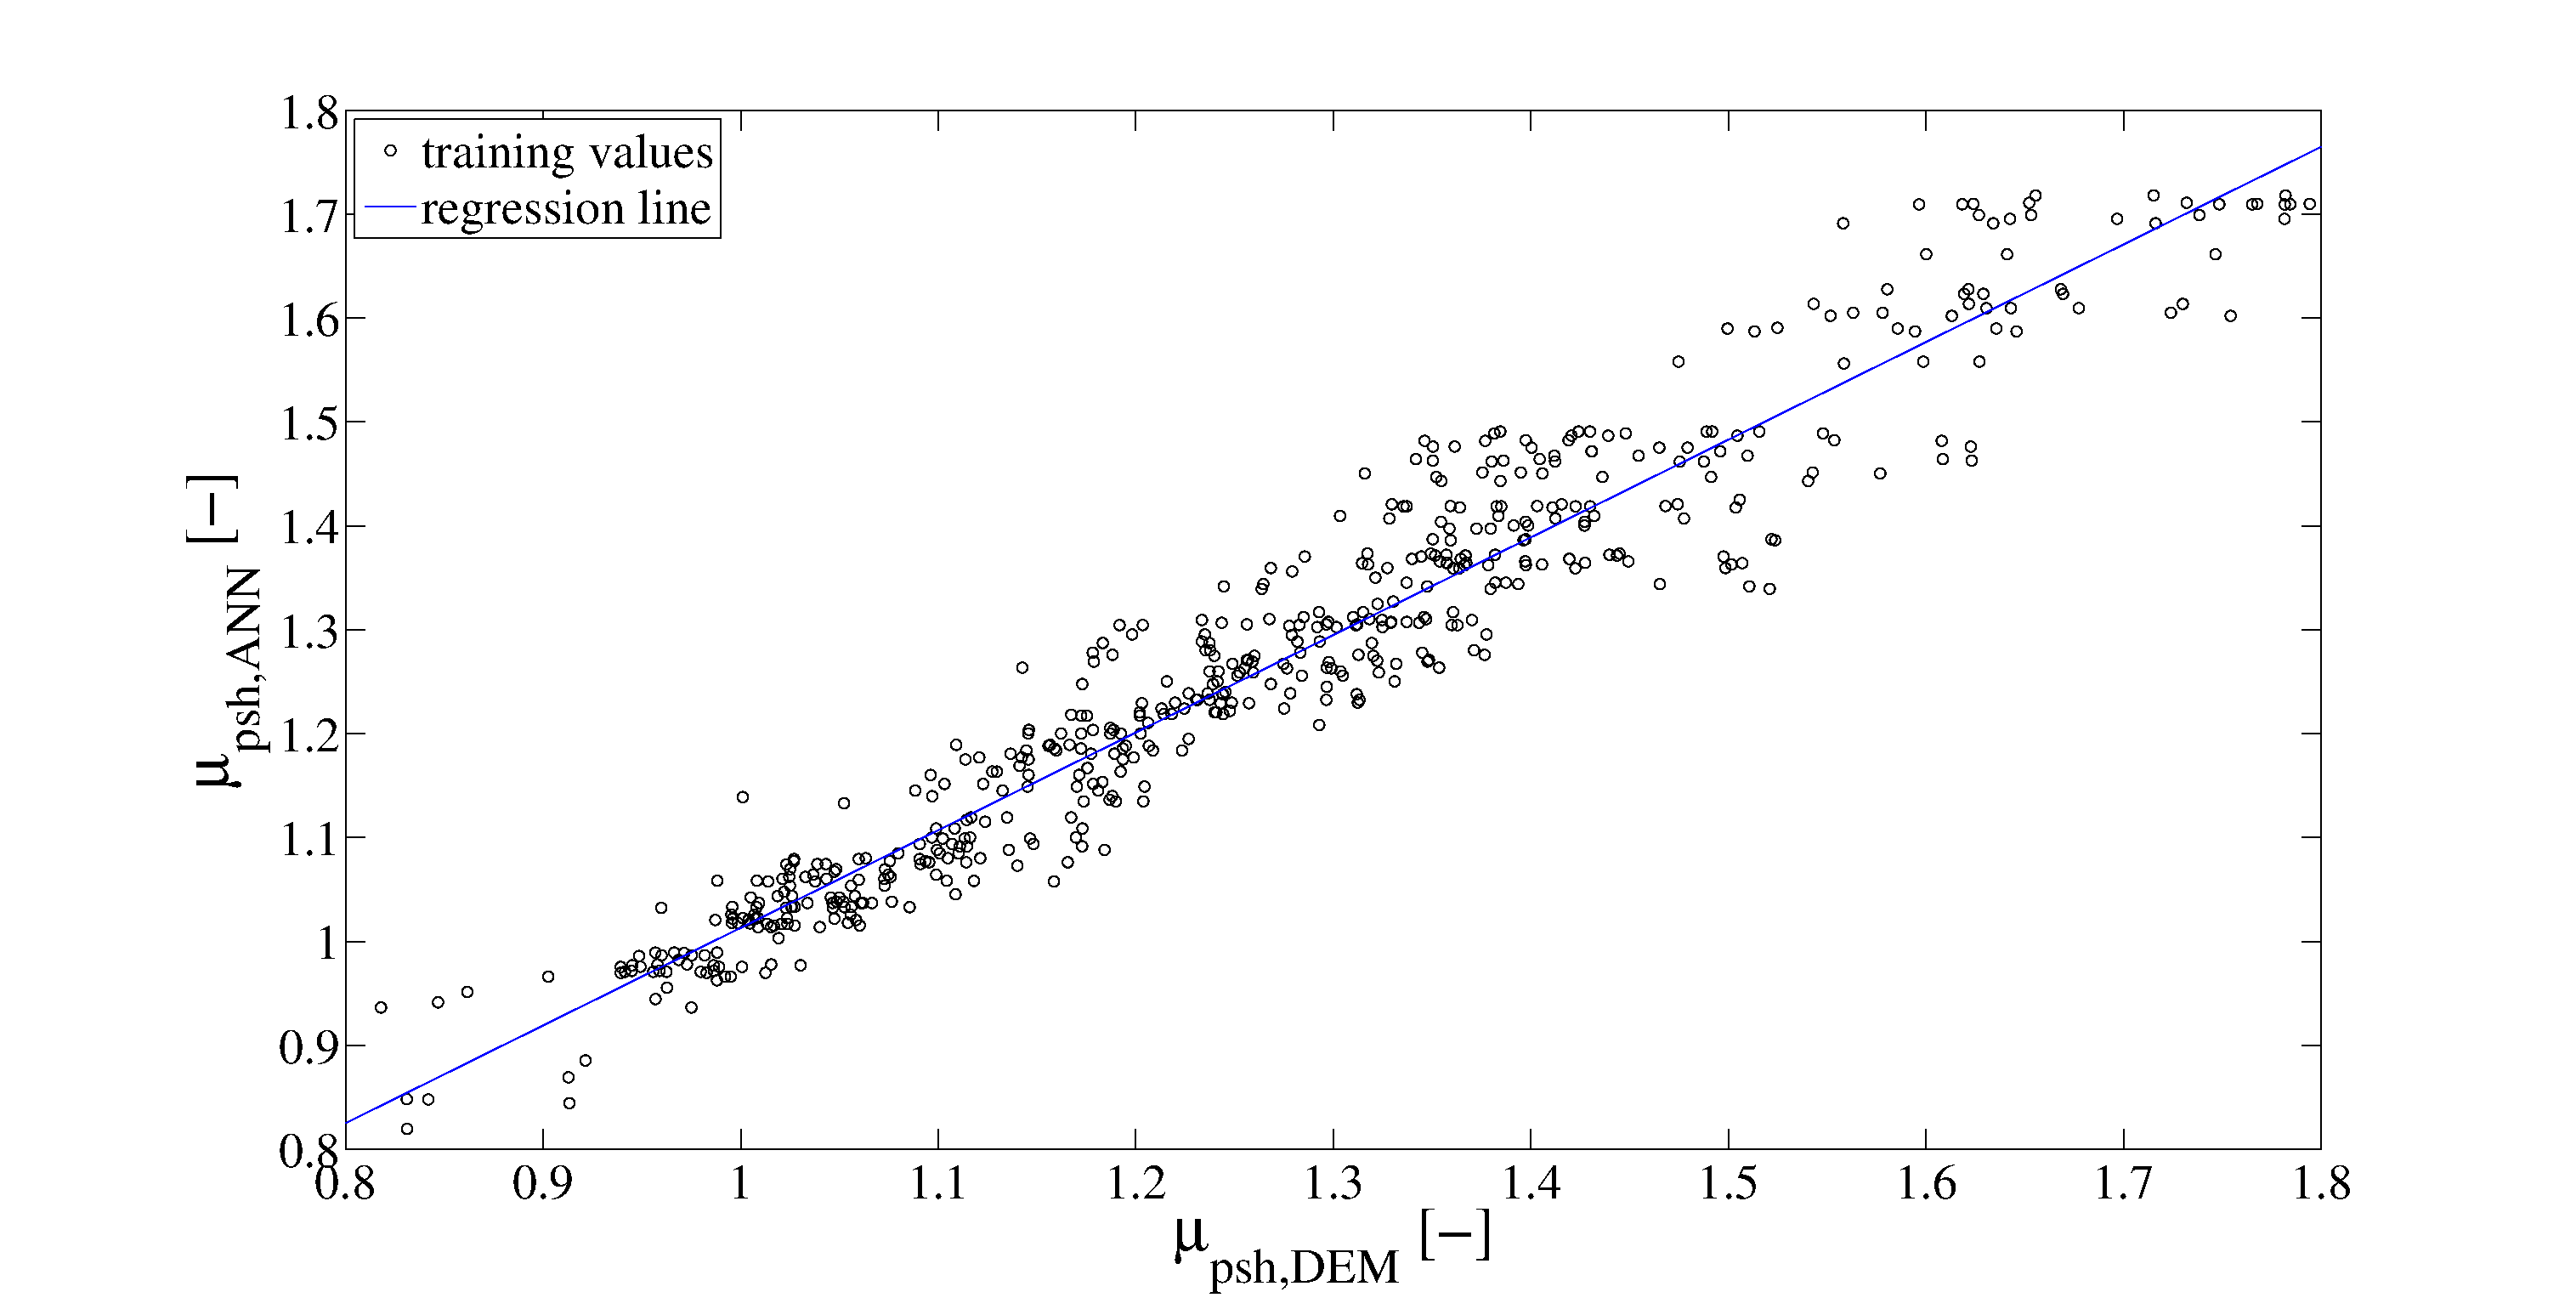
\includegraphics[width=.80\columnwidth]{images/022regression.eps}
% %[width=.48\textwidth]
% \caption[Comparison between prediction of the trained ANN and full DEM
% simulation]{Comparison between prediction of the trained Artificial Neural
% Network ($ANN$) and 546 
% \wrong{write down all the simulations performed at the end.}
% full DEM simulations of the coefficient of pre-shear
% (\ac{mupsh}).}
% \label{fig:022regression} 
% \end{figure}
%************************************************

\section{Experiments and Parameter Identification}
\label{sec:experimentsparameteridentification}

\begin{table}[h]
\centering
\begin{tabular}{ccc}
\hline
    Young's & Poisson's & \acs{deltat}\\
   modulus & ratio & \\
    $[MPa]$ & $[-]$ & [s]\\
    \hline
    $10$    & $0.40$ & $10^{-6}$\\


\hline
\end{tabular}
\caption{DEM fixed input values}
\label{tab:09DEMFixedinputvalues}
\end{table}


Experimental values identifying the bulk behavior, $\mu_{psh}$, $\mu_{sh}$ and $\rho_{b}$, 
of sinter fine were acquired through $SSC$ tests. 
Table \ref{tab:05sinterTableExperimental} presents
these values for three load conditions: clearly the $\mu_{psh}$ decreases, and 
the $\mu_{sh}$ oscillates.
The $\rho_b$ has a clear average of 1,760 $kg/m^3$ with a 42 
$kg/m^3$ deviation.
Two $AoR$ tests were performed that gave an average angle of
38.85$^\circ$.
We obtained the radius ($R$) mean and standard
deviations, as shown in Table
\ref{tab:09DEMFixedinputvalues}, from sieving experiments.
The comparison between numerical and experimental behaviours led to a first
series of marked combinations ($MC1$) for one load condition of
the shear cell ($\sigma_n=10,070$ Pa, P=1.0), as plotted in Fig.
\ref{fig:024radarpirker1schulze10070}, where 
the minimum and maximum values are shown, together with the mean. 
Each axis of the parameter space plot represents one simulation parameter.
The shaded area indicates valid parameter combinations, and dark shaded
values indicate the confidence range.
Note that the confidence interval is large, 
especially for the $COR$, which highlights its insignificant influence on the
characterization.
Both the $\rho_p$  and the $\mu_s$, however, show a narrow confidence interval, 
which demonstrates their influence and the ability of this procedure to find
valid $DEM$ parameters.
These results agree with our examination of the ratio of the standard deviation
to the range, see Table \ref{tab:13DEMvalidvalues}.
Further, we observed that various $DEM$ parameter
combinations could reproduce the experimental behaviour, and thus evaluated
their mutual dependencies.
This is shown more clearly in a density plot (see Fig. 
\ref{fig:025cloudpirker1schulze10070} for $MC1$) 
of the particles' coefficient of restitution ($COR$) in relation to
the coefficients of sliding friction ($\mu_s$) and rolling friction ($\mu_r$); 
in the white area, no valid sets of simulation parameters can be found.
In each cell the valid sets are grouped according to the 4 different COR
ranges.
Each cell is coloured according to the group with the most members.
Multiple
combinations (250,407 or 4\% of the total) of $\mu_s$ and $\mu_r$ reproduced
the experimental behaviour with varying $COR$.
This underlines once more their correlation, as already stated by Wensrich and 
Katterfeld \cite{RefWorks:87}.
To further demonstrate the validity of the procedure, we modified the product
coefficient. 
First, we set it to $P=0.8$, and we obtained another
series of marked combinations ($MC2$).
It can be seen in the parameter space plot in Fig.
\ref{fig:026radarpirker08schulze10070} that the confidence range is narrower
than for $P=1.0$, while in the density plot in Fig. 
\ref{fig:027cloudpirker08schulze10070} the area
appears larger, although slightly less densely populated. Finally, for $P=1.2$
and its marked combinations ($MC3$) the parameter space plot in Fig.
\ref{fig:028radarpirker12schulze10070} shows a largely different confidence
range, while the density plot in Fig. \ref{fig:030cloudpirker12schulze10070} 
shows a smaller area. As expected, the procedure was highly sensitive to
variations in the experimental data.
Our approach could therefore be used
for a wide range of bulk materials.\\
We then processed the random combinations with the $AoR$ $ANN$. In Fig.
\ref{fig:031radarpirker1aor} the parameter space plot for the same criteria as
before can be seen.
In accordance with theory (Wensrich and Katterfeld \cite{RefWorks:87}), in a simulation dominated
by rolling particles, the coefficient of rolling friction has the maximum
influence. \\
Finally, we extracted from the $MC1$ values the $AoR$ $ANN$ behaviour
and compared it with the experimental one.
As can be seen in the parameter space plot in Fig.
\ref{fig:033radarpirker1schulze10070aor}, the confidence interval is very small,
indicating that all the parameters but the $COR$ played an important role, 
and demonstrating the reliability of these parameter
combinations in representing the bulk behaviour.
From the initial 6,250,000 combinations, only 3,884 were valid (0.0621
\%), see Table \ref{tab:13DEMvalidvalues}.
%************************************************
\begin{table}[h]
\centering
\begin{tabular}{cccccc}
\hline
$\sigma_n$ (Pa) & $\tau$ (Pa) & $\mu_{psh}$ (-) & $\tau_{\%}$ (\%) &
$\mu_{sh}$ (-) & $\rho_b$ (kg/m3) \\
\hline
    1068  & 1059  & 0.9916 & 80 & 1.2333 & 1718 \\
    2069  & 1818  & 0.8787 & 80 & 0.9994 & 1759 \\
    10070 & 8232  & 0.8175 & 80 & 1.1712 & 1802 \\

\hline
\end{tabular}
\caption[Experimental results]{Experimental results. Values for three
load conditions}
\label{tab:05sinterTableExperimental}
\end{table}

\begin{table}[h]
\centering
\begin{tabular}{llccc}
\hline

          & type  & SSC & AoR   & SSC \& AoR \\
          \hline

    $\mu_s$ & mean  & 0.831 & 0.177 & 0.664 \\
    $[-]$   & std. dev. (SD) & 0.097 & 0.095 & 0.029 \\
          & range ($R$) & 0.9   & 0.9   & 0.9 \\
          & SD / R & 0.108 & 0.106 & 0.032 \\
          \hline
    $\mu_r$ & mean  & 0.692 & 0.830 & 0.916 \\
    $[-]$   & std. dev. (SD) & 0.215 & 0.193 & 0.042 \\
          & range ($R$) & 0.9   & 0.9   & 0.9 \\
          & SD / R & 0.239 & 0.214 & 0.046 \\
          \hline
              COR   & mean  & 0.708 & 0.590 & 0.590 \\
   $ [-]$   & std. dev. (SD) & 0.104 & 0.073 & 0.065 \\
          & range ($R$) & 0.4   & 0.4   & 0.4 \\
          & SD / R & 0.259 & 0.183 & 0.161 \\
          \hline
    $\rho_p$ & mean  & 2245.7 & 3192.8 & 2283.9 \\
    $[kg/m3]$ & std. dev. (SD) & 80.5  & 277.4 & 67.1 \\
          & range ($R$) & 1500  & 1500  & 1500 \\
          & SD / R & 0.054 & 0.185 & 0.045 \\
          \hline
    valid & number & 290203 & 816552 & 3884 \\
    combinations & [$\%$] & 4.64  & 13.06 & 0.06 \\  

\hline
\end{tabular}
\caption[DEM valid values]{DEM valid values. For each parameter we show the
valid parameters statistics in the two tests and in their intersection.
Finally, we show the number of valid parameters combinations over the total
(6250000).}
\label{tab:13DEMvalidvalues}
\end{table}


%************************************************
\begin{figure}[htbp]
\centering 
  \subfloat[Parameter space plot, \acs{SCT}, $\sigma_n=1068$ Pa, P=1.0.]{
	  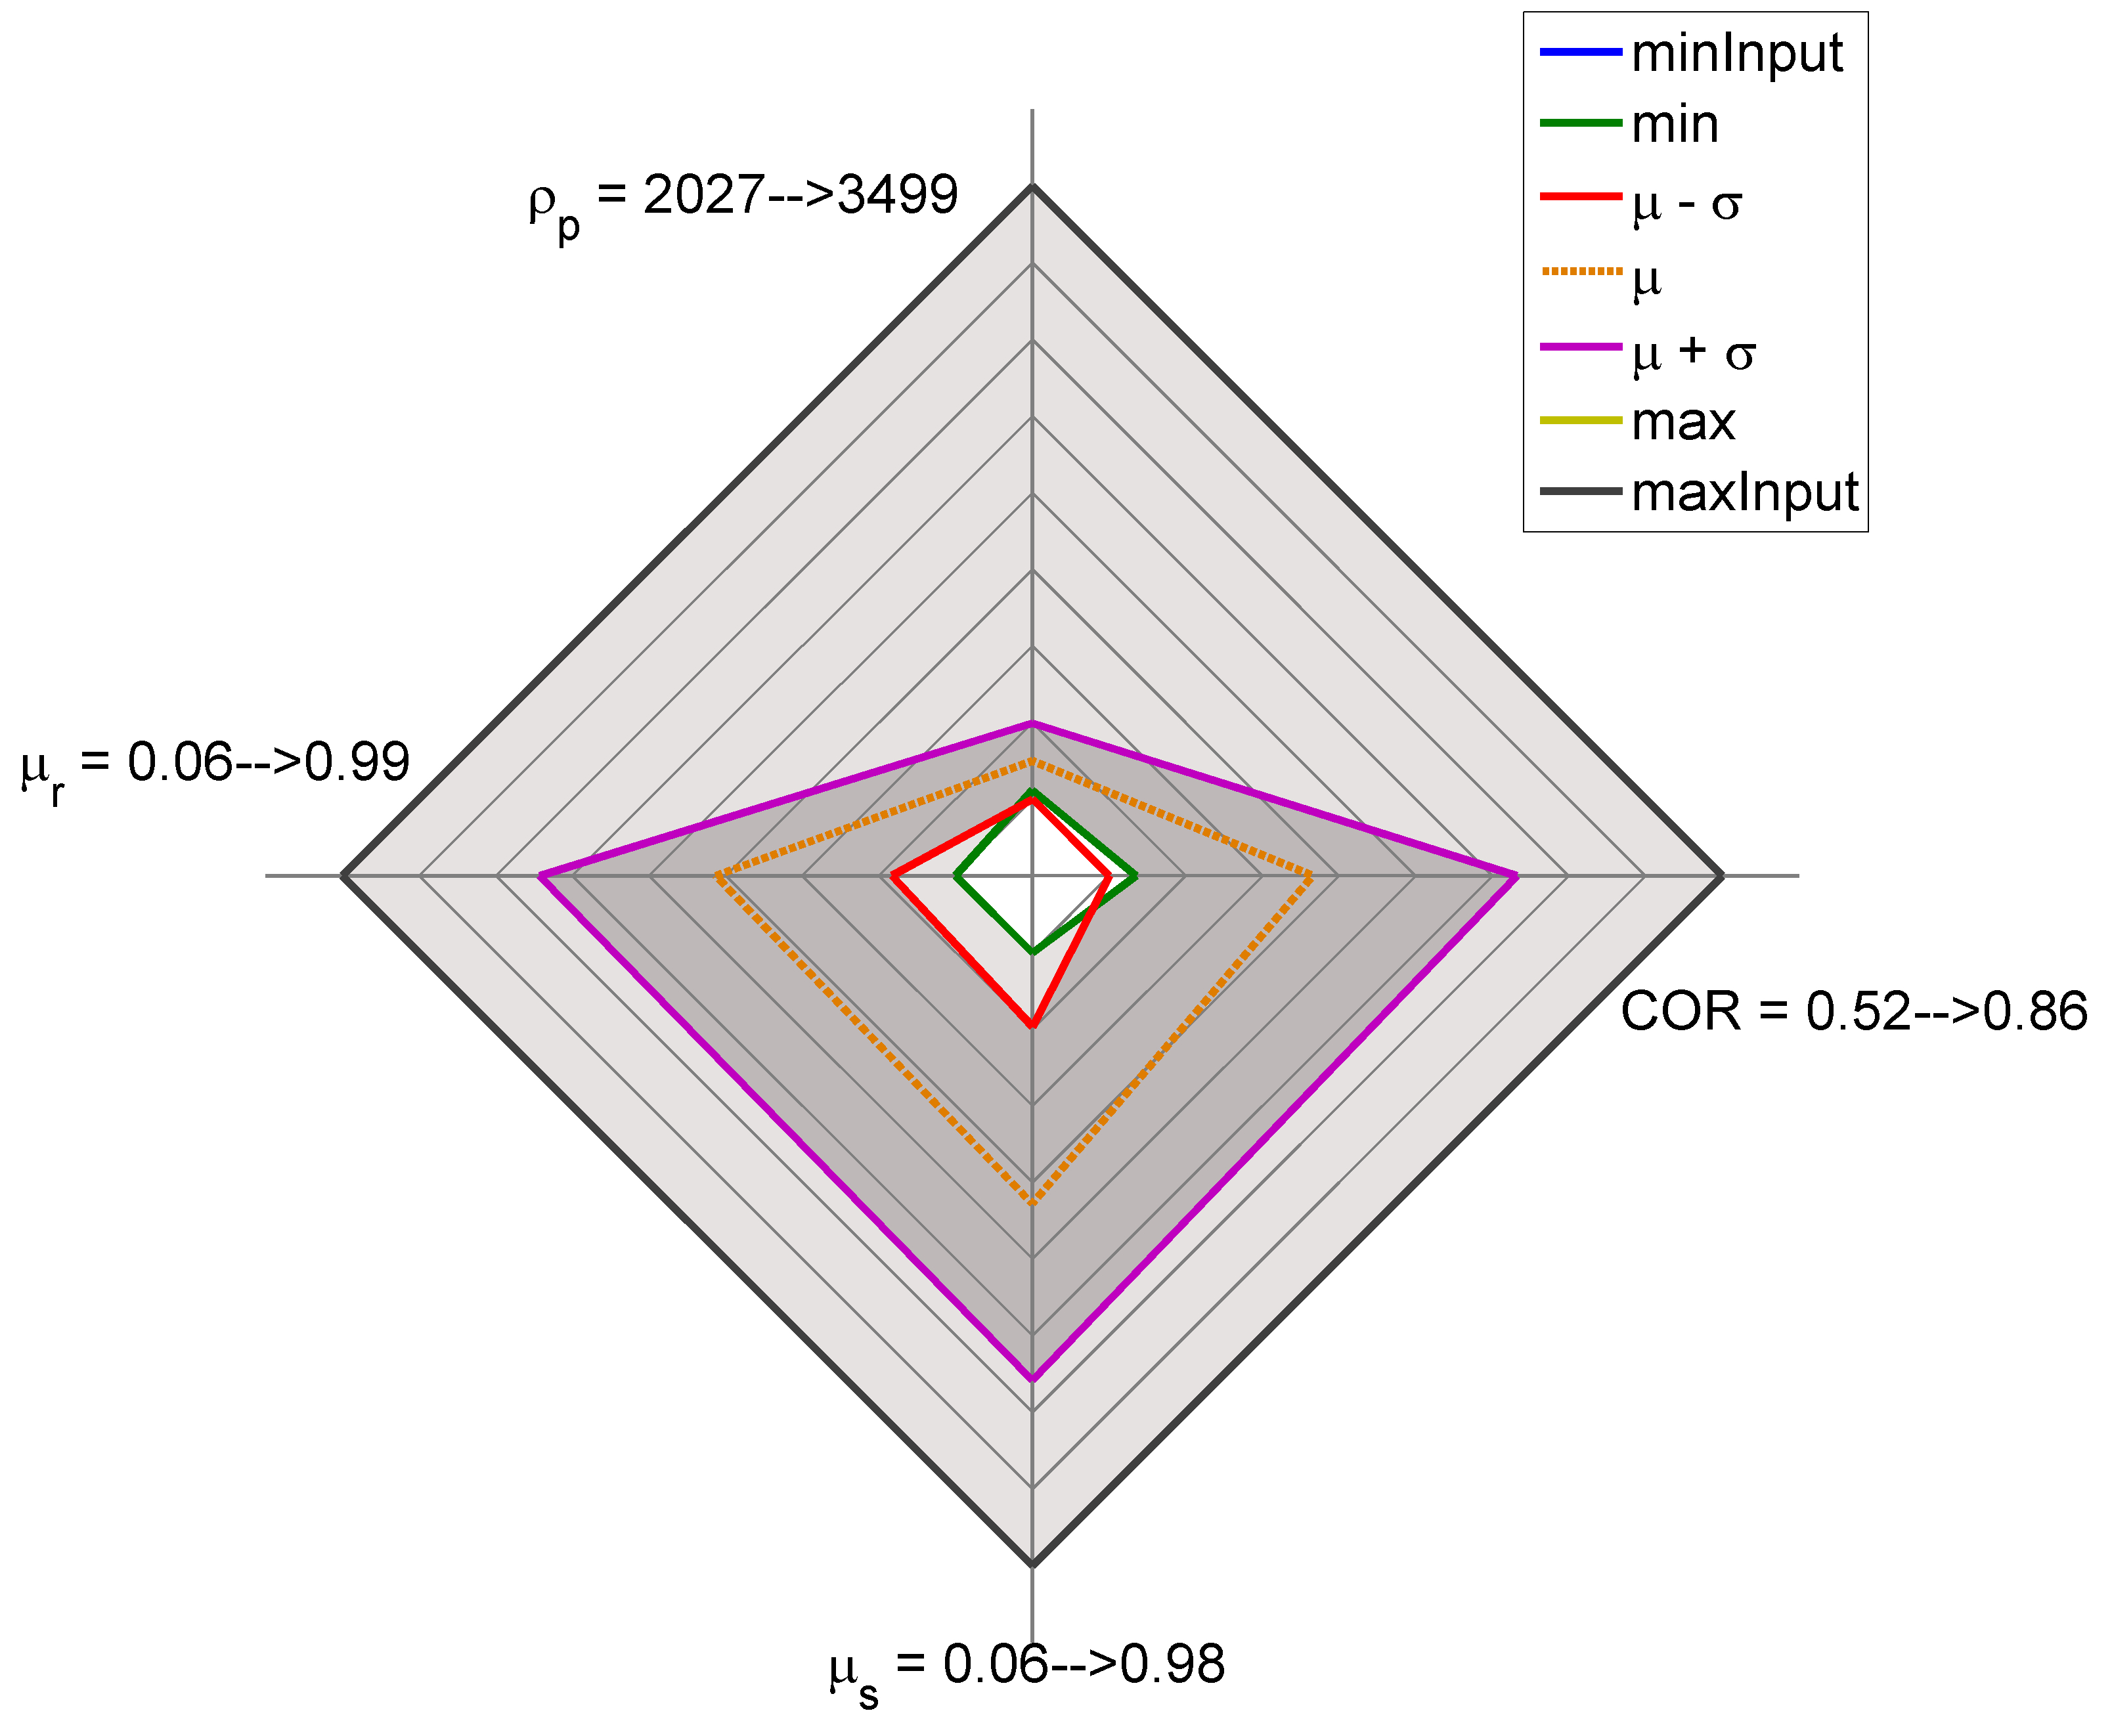
\includegraphics[width=.35\columnwidth]{images/041radarpirker1schulze1068}
	  \label{fig:041radarpirker1schulze1068}
  }
  \\
    \subfloat[Parameter space plot, \acs{SCT}, $\sigma_n=10070$ Pa, P=0.8.]{
	  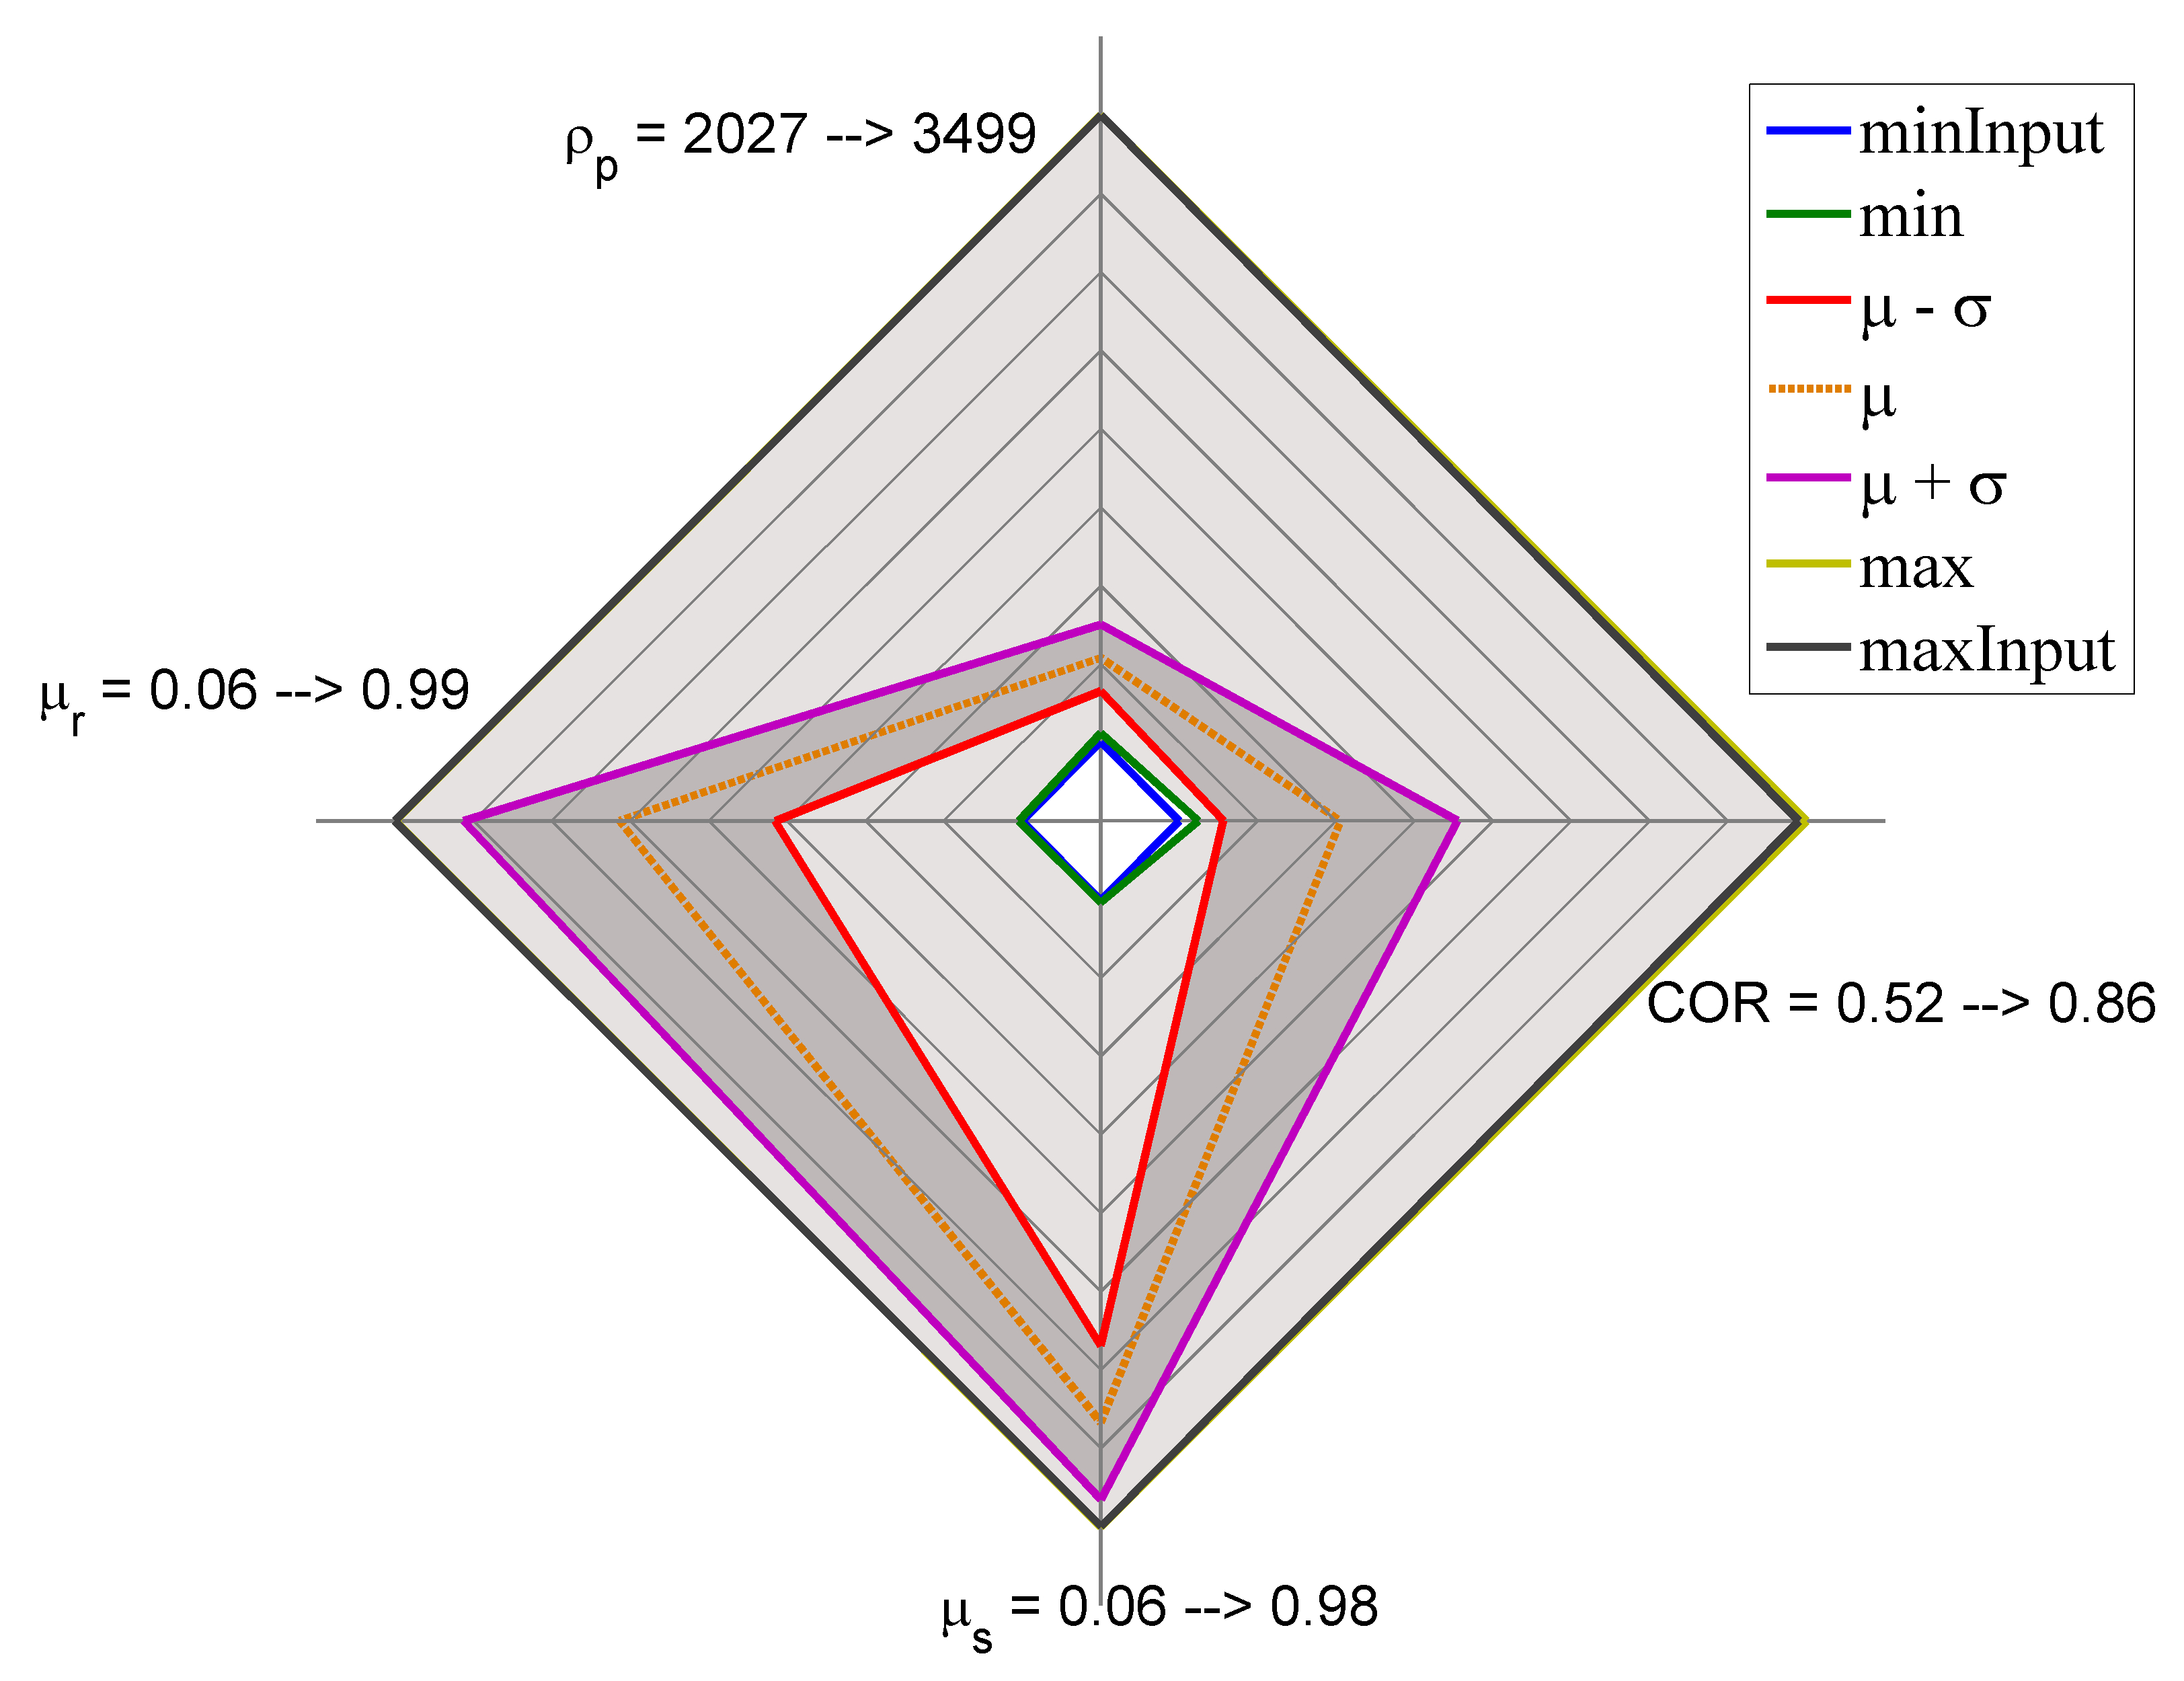
\includegraphics[width=.35\columnwidth]{images/026radarpirker08schulze10070}
	  \label{fig:026radarpirker08schulze10070}
  }
  \\
  \subfloat[Parameter space plot, \acs{SCT}, $\sigma_n=10070$ Pa, P=1.0.]{
	  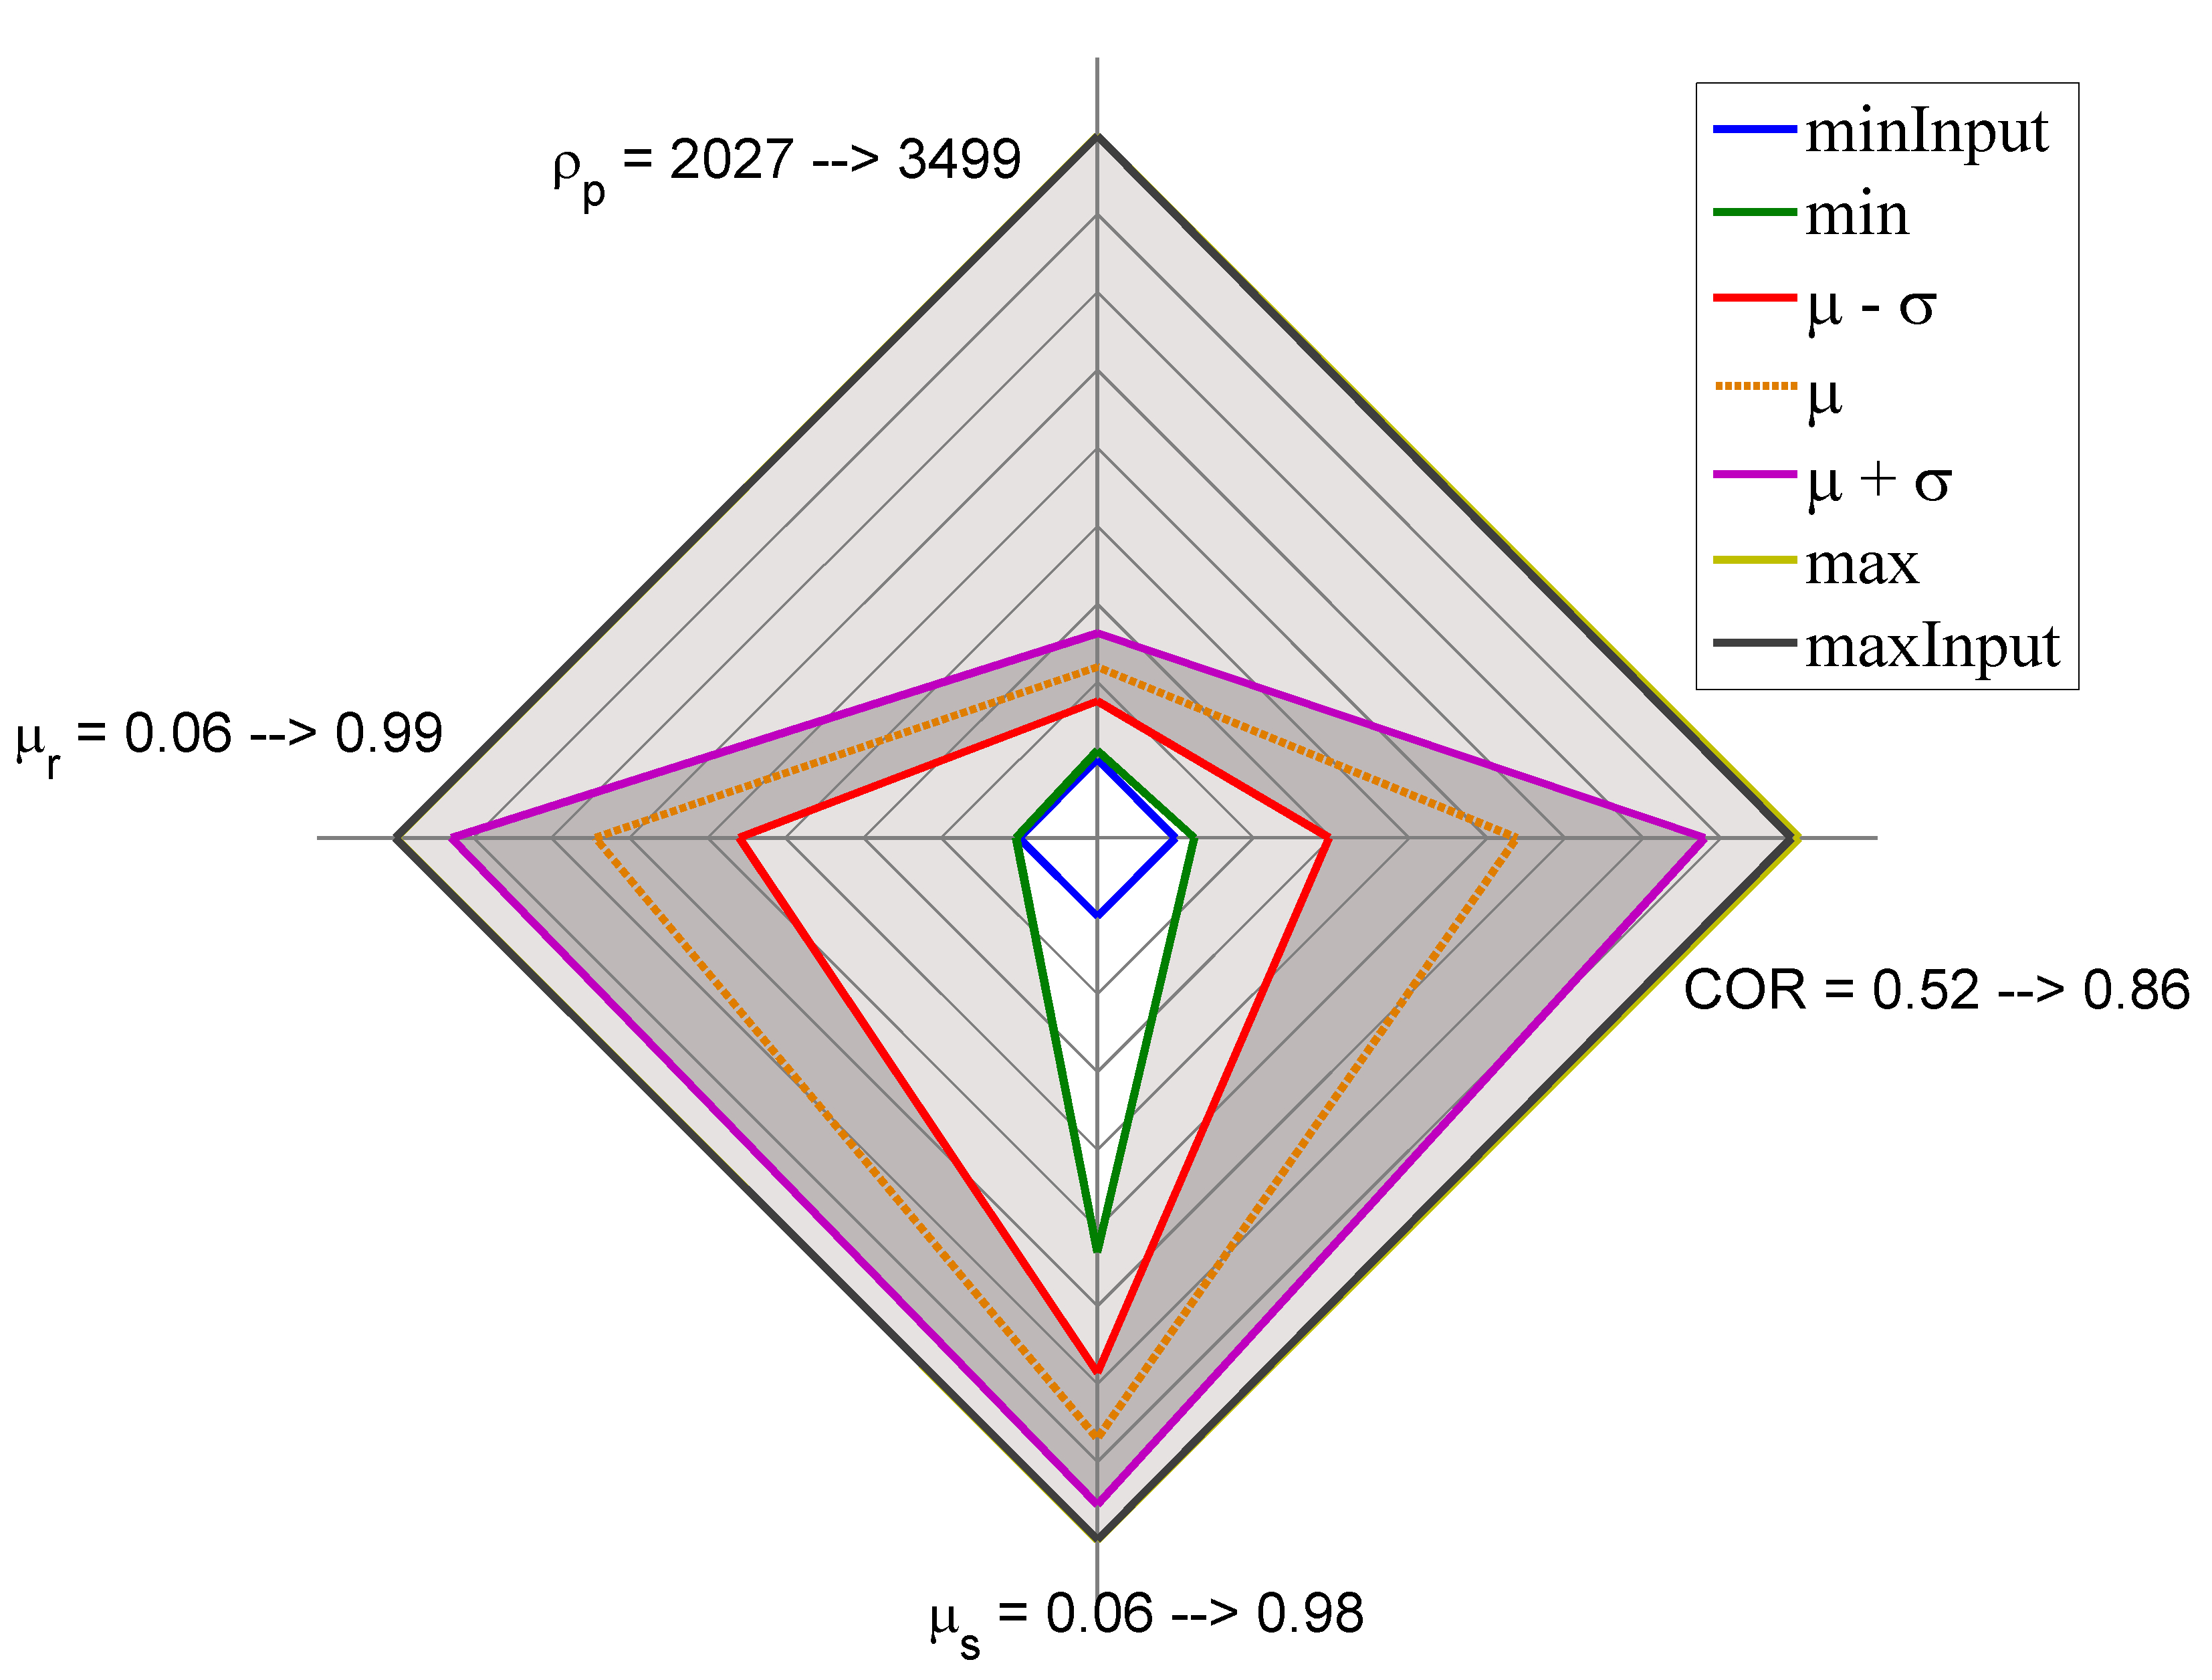
\includegraphics[width=.35\columnwidth]{images/024radarpirker1schulze10070}
	  \label{fig:024radarpirker1schulze10070}
  }
  \quad
    \subfloat[Box plot, \acs{SCT}, $\sigma_n=10070$ Pa, P=1.0.]{
	  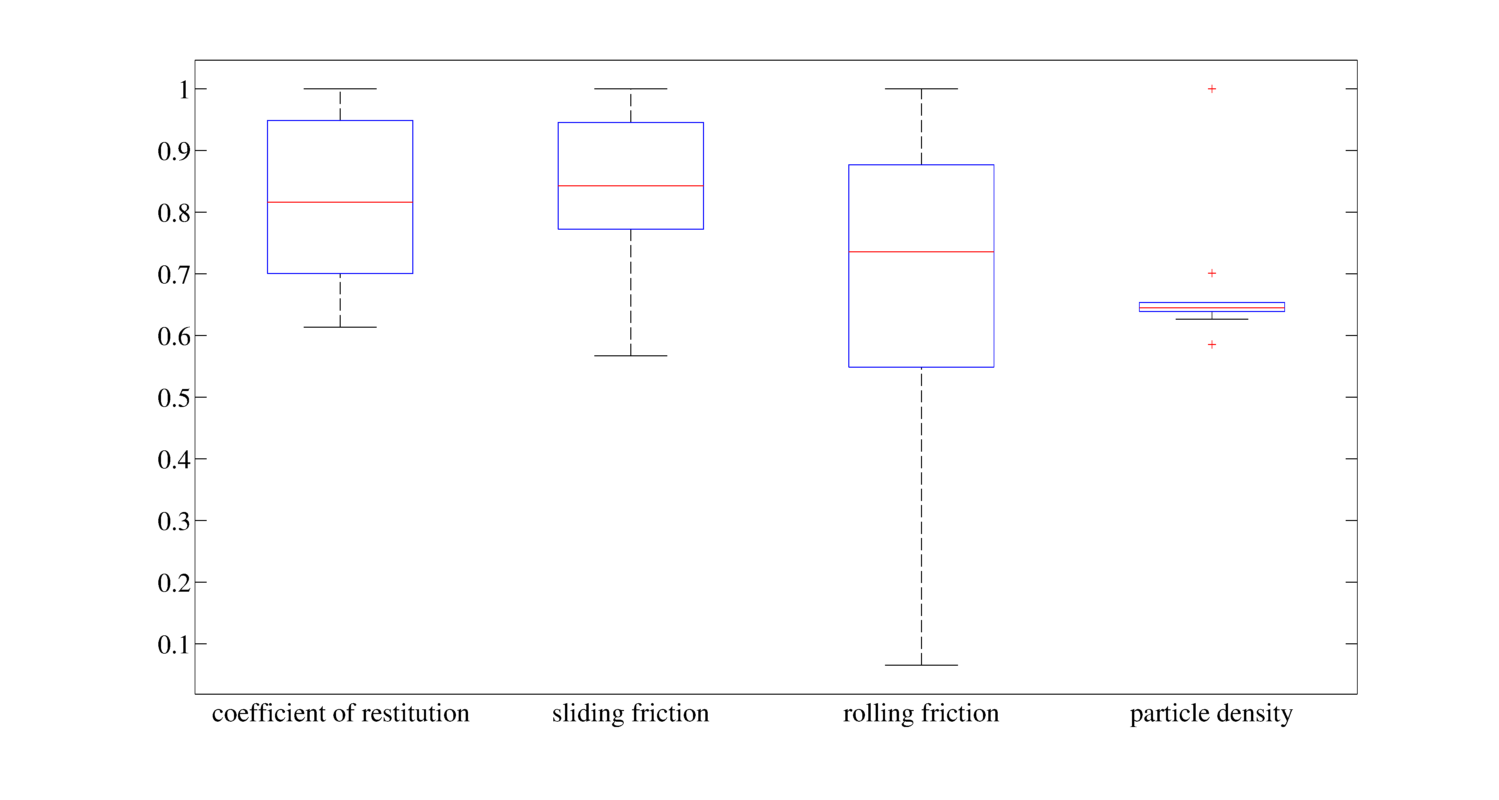
\includegraphics[width=.35\columnwidth]{images/075sctboxplot}
	  \label{fig:075sctboxplot}  }
  \\
    \subfloat[Parameter space plot, \acs{SCT}, $\sigma_n=10070$ Pa, P=1.2.]{
	  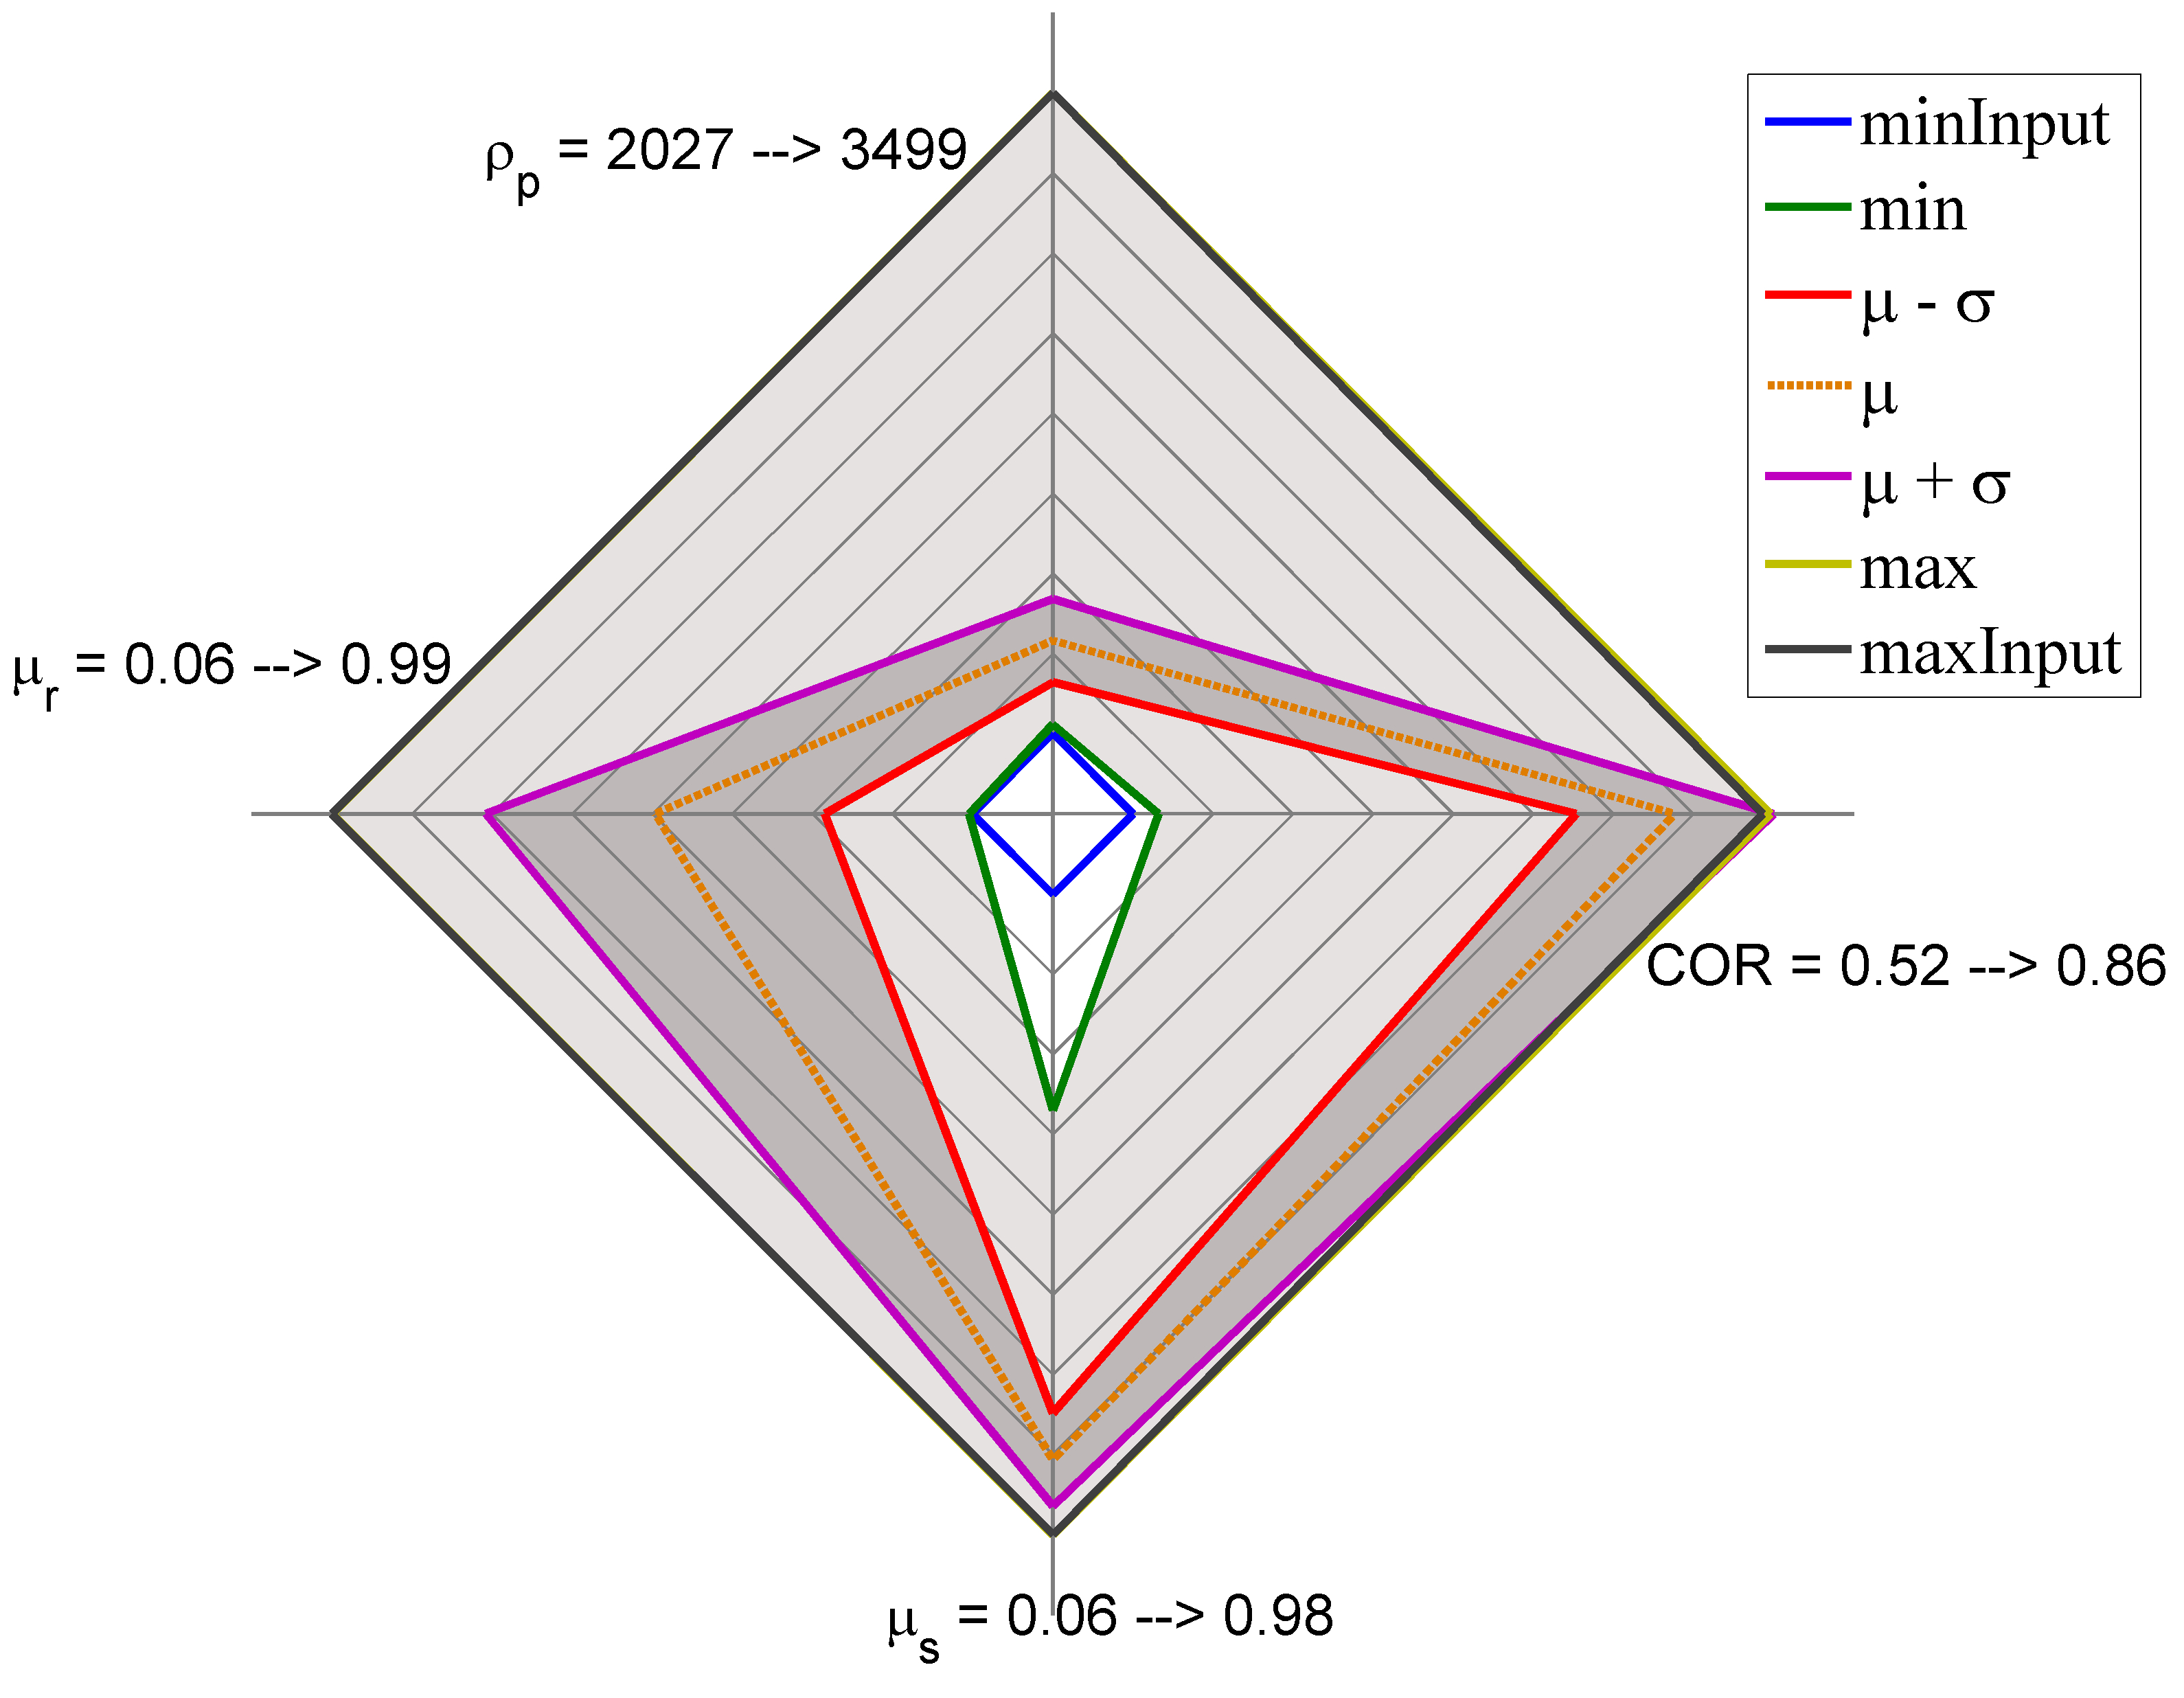
\includegraphics[width=.35\columnwidth]{images/028radarpirker12schulze10070}
	  \label{fig:028radarpirker12schulze10070}
  }
  \caption{SCT parameter space plots.}
  \label{fig:079sctparameterspaceplots}
\end{figure}
\begin{figure}[htbp]
\centering 
  \subfloat[Density plot, $SSC$, $\sigma_n=10070$ Pa, P=0.8.]{
	  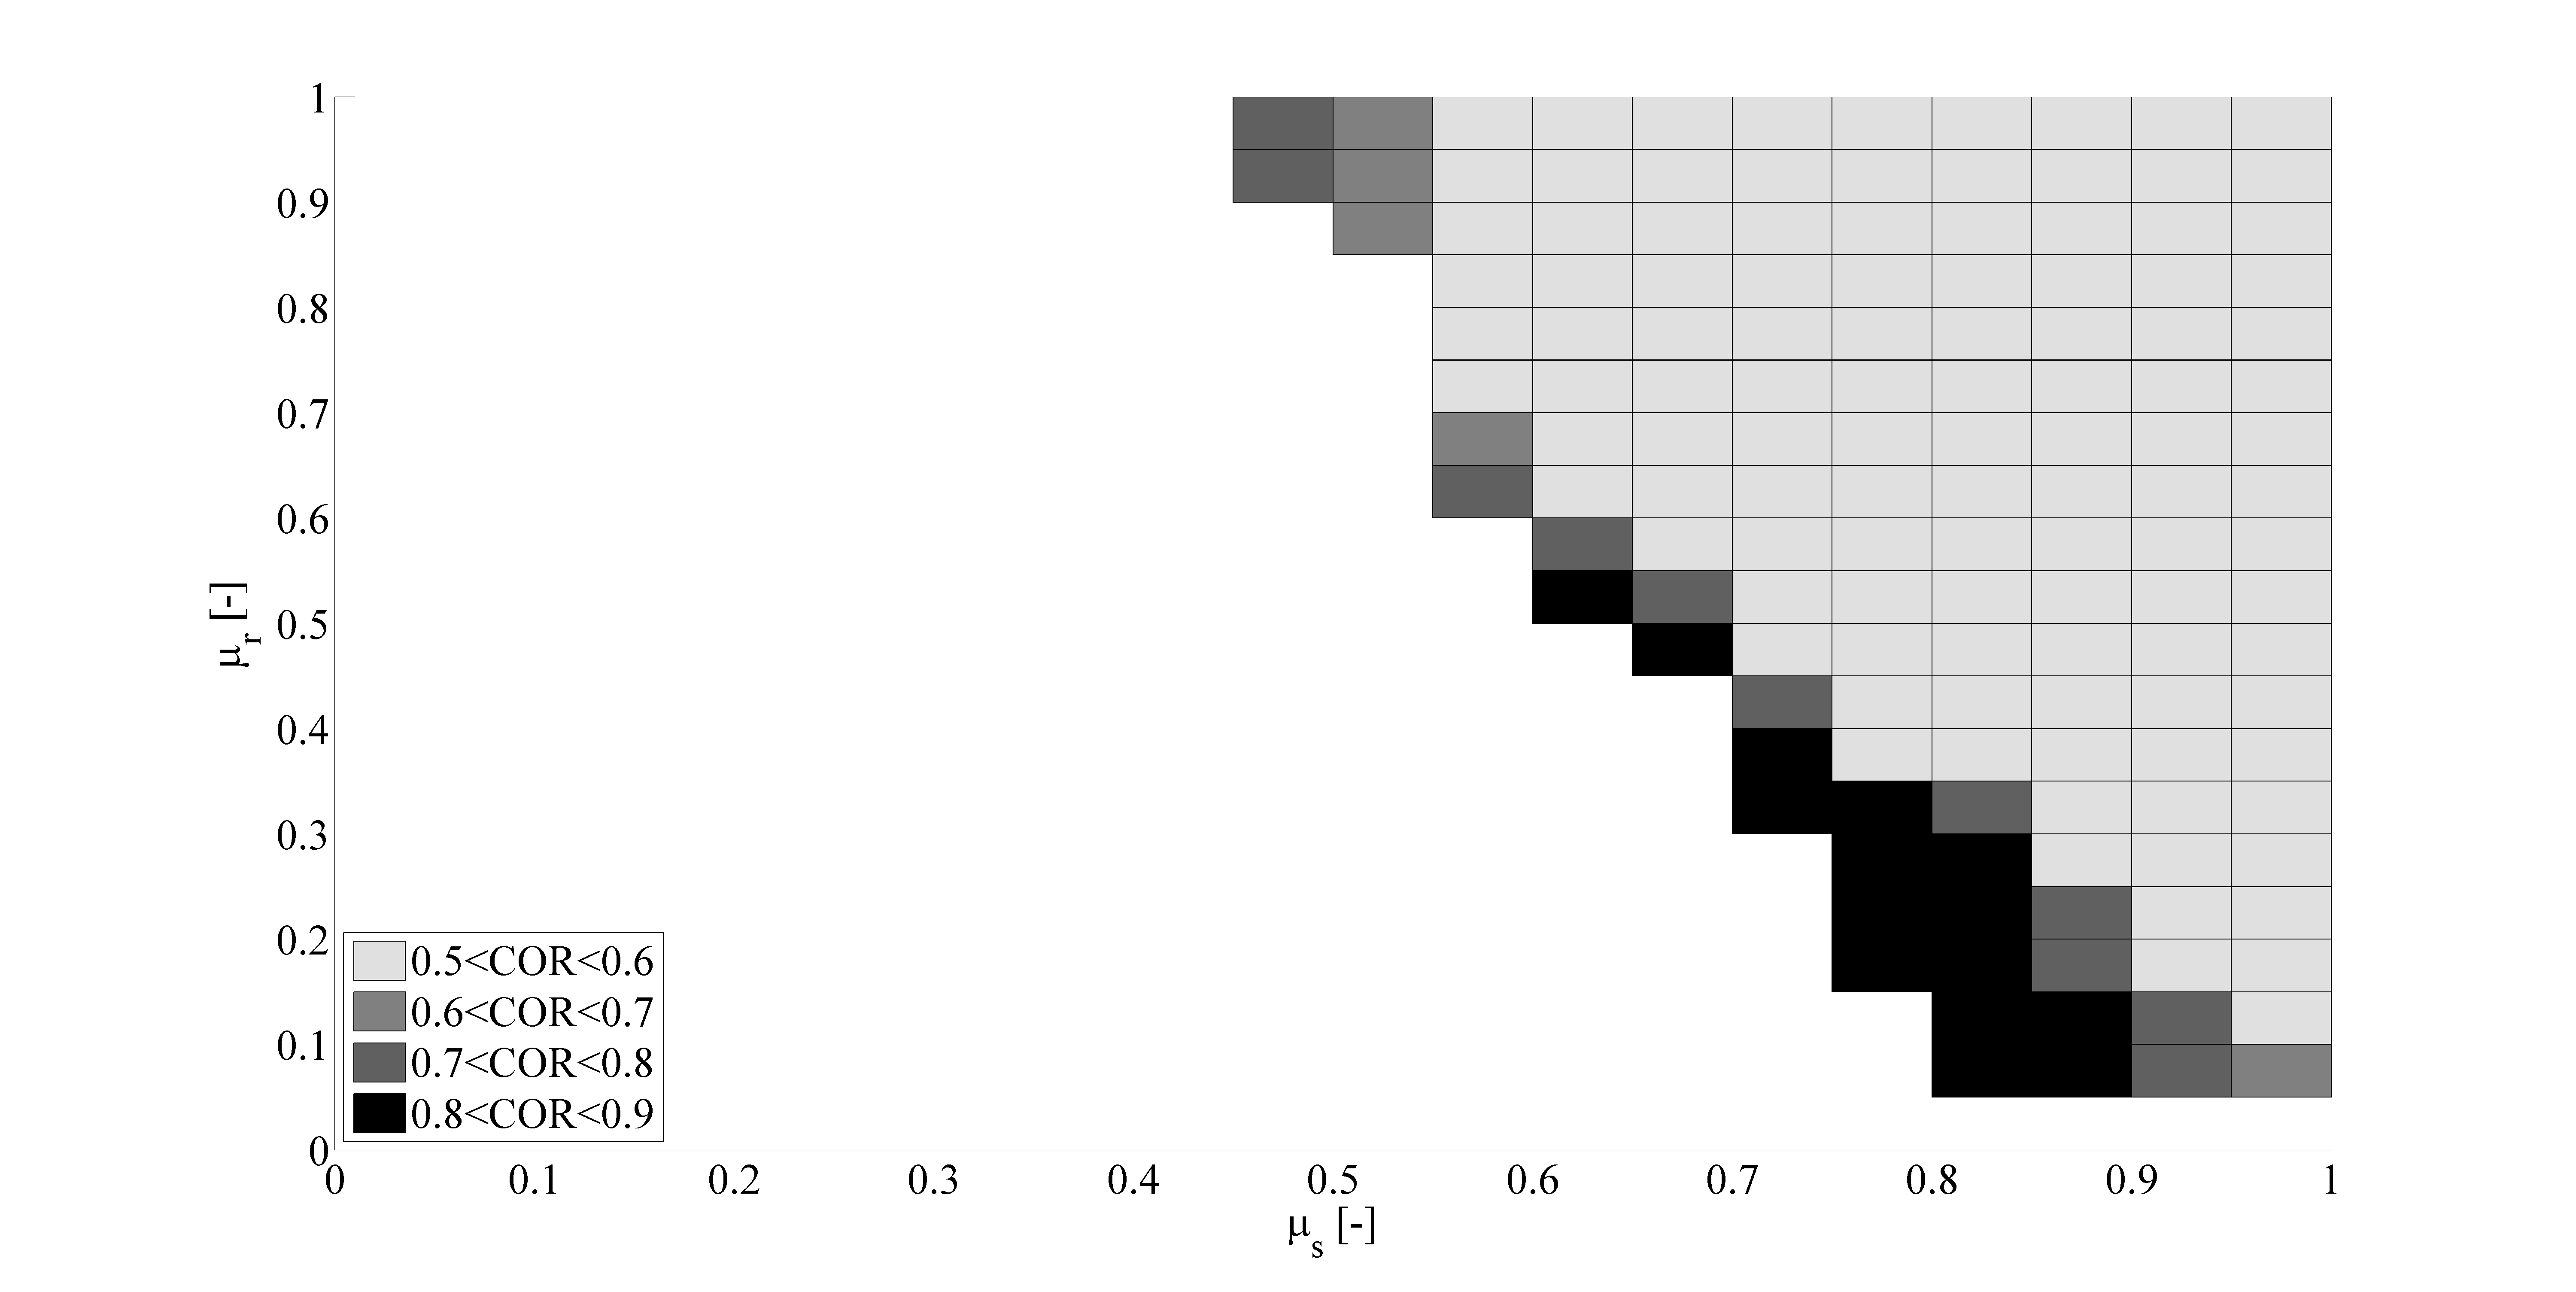
\includegraphics[width=.48\columnwidth]{images/027cloudpirker08schulze10070}
	  \label{fig:027cloudpirker08schulze10070}
  }
  \\
    \subfloat[Density plot, $SSC$, $\sigma_n=10070$ Pa, P=1.0.]{
	  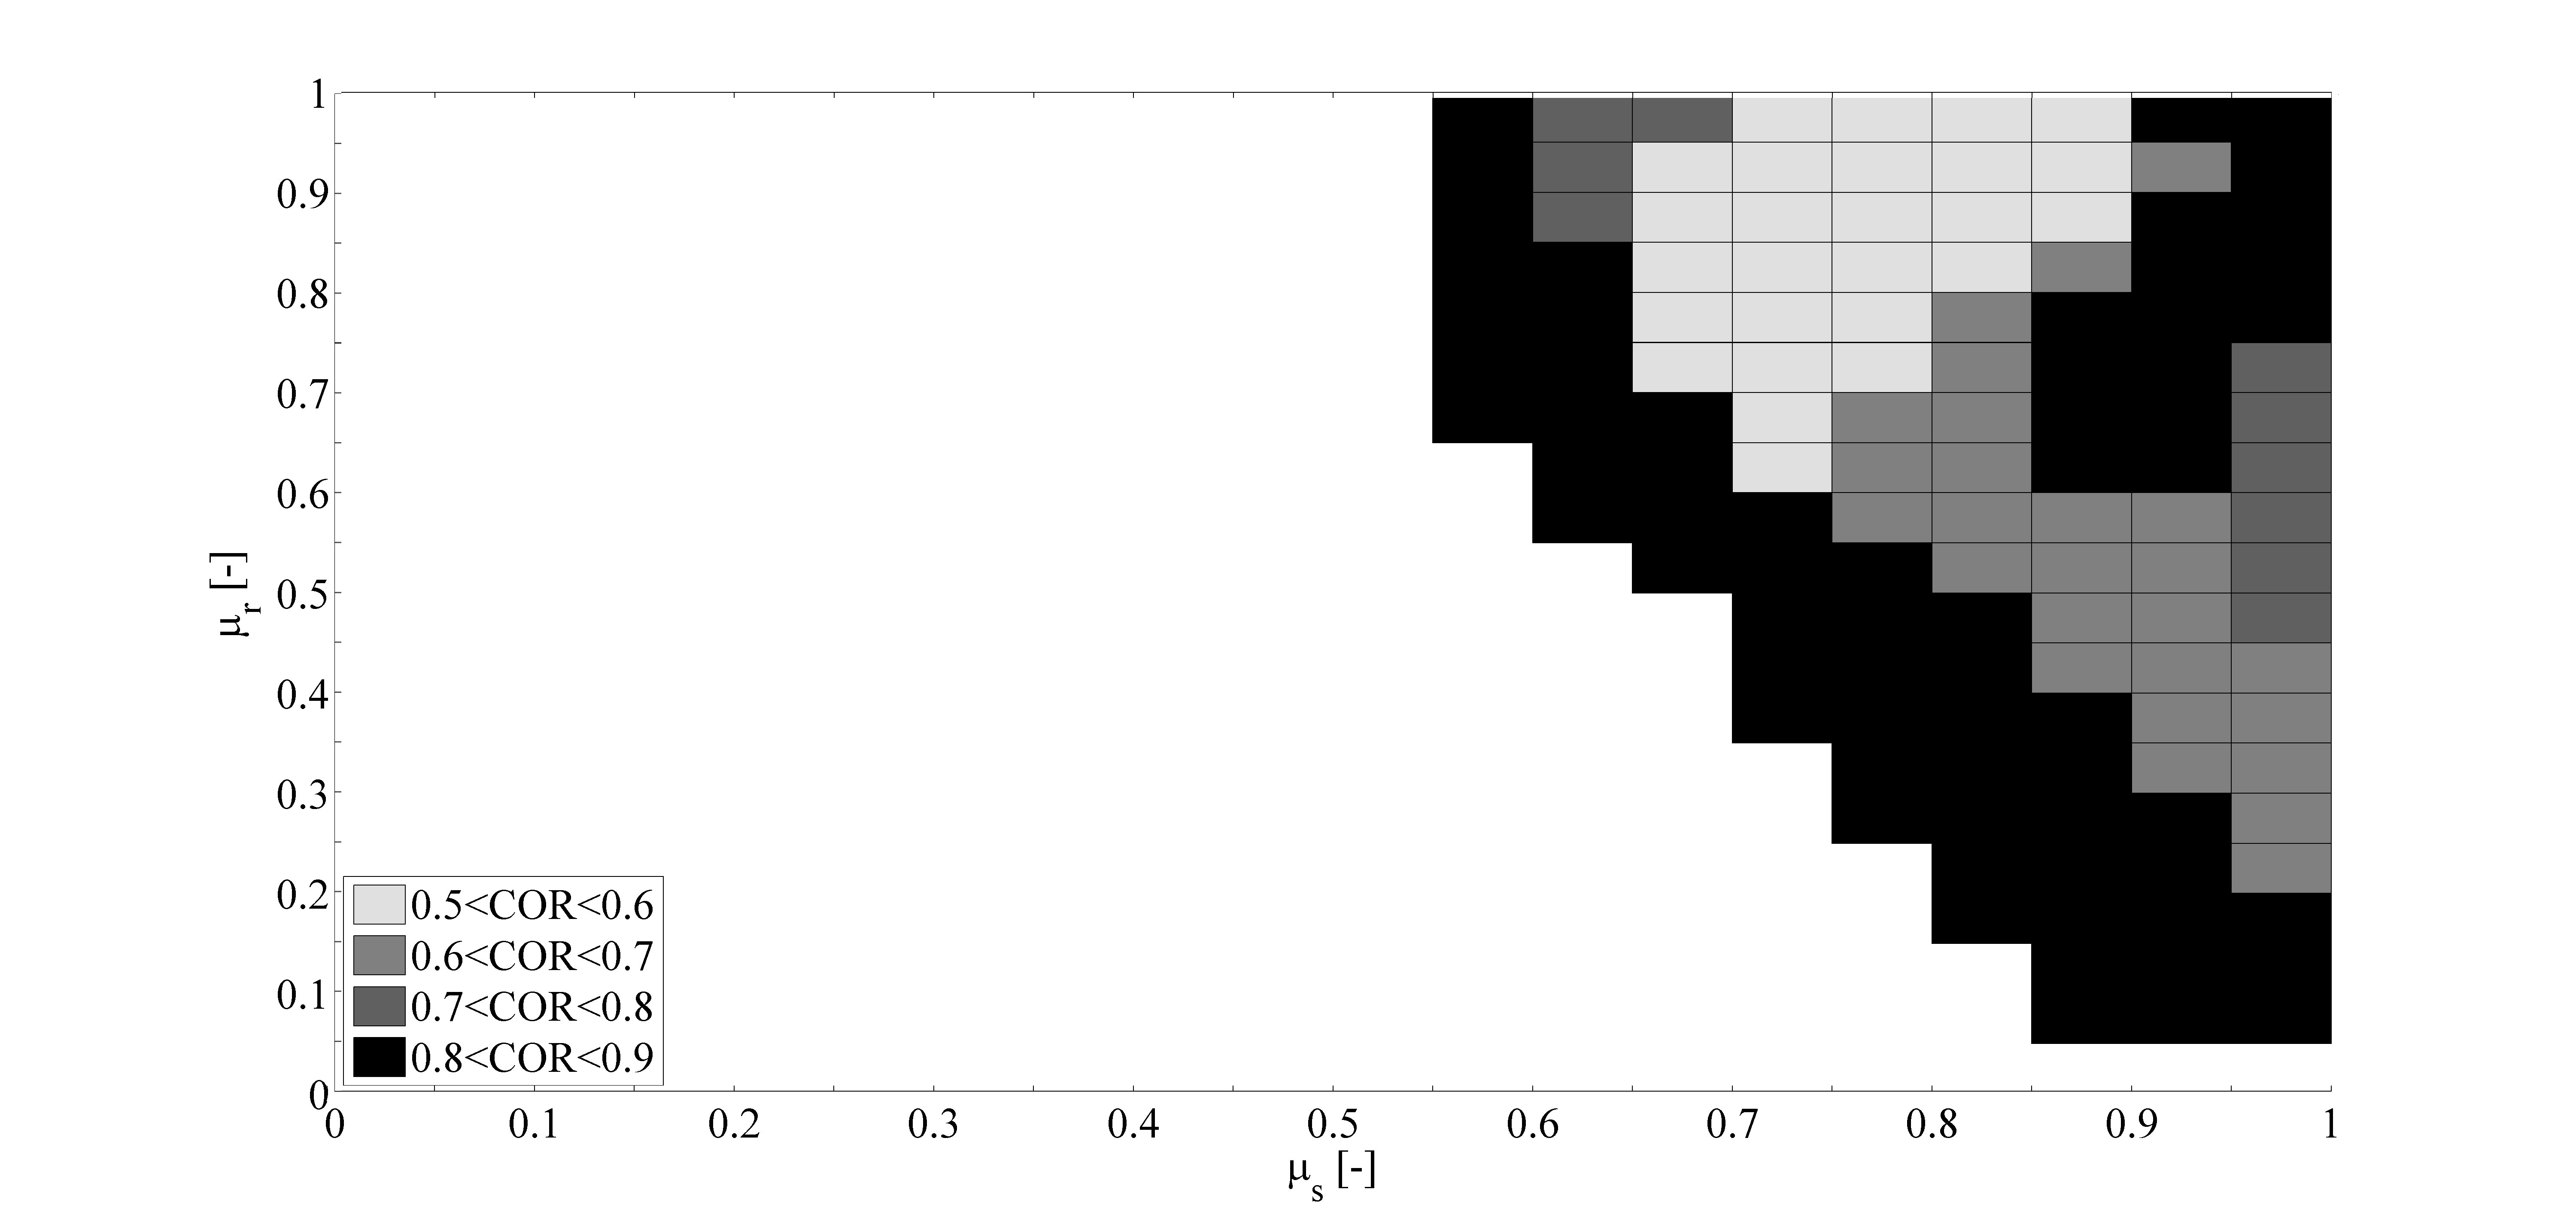
\includegraphics[width=.48\columnwidth]{images/025cloudpirker1schulze10070}
	  \label{fig:025cloudpirker1schulze10070}
  }
  \\
  \subfloat[Density plot, $SSC$, $\sigma_n=10070$ Pa, P=1.2.]{
	  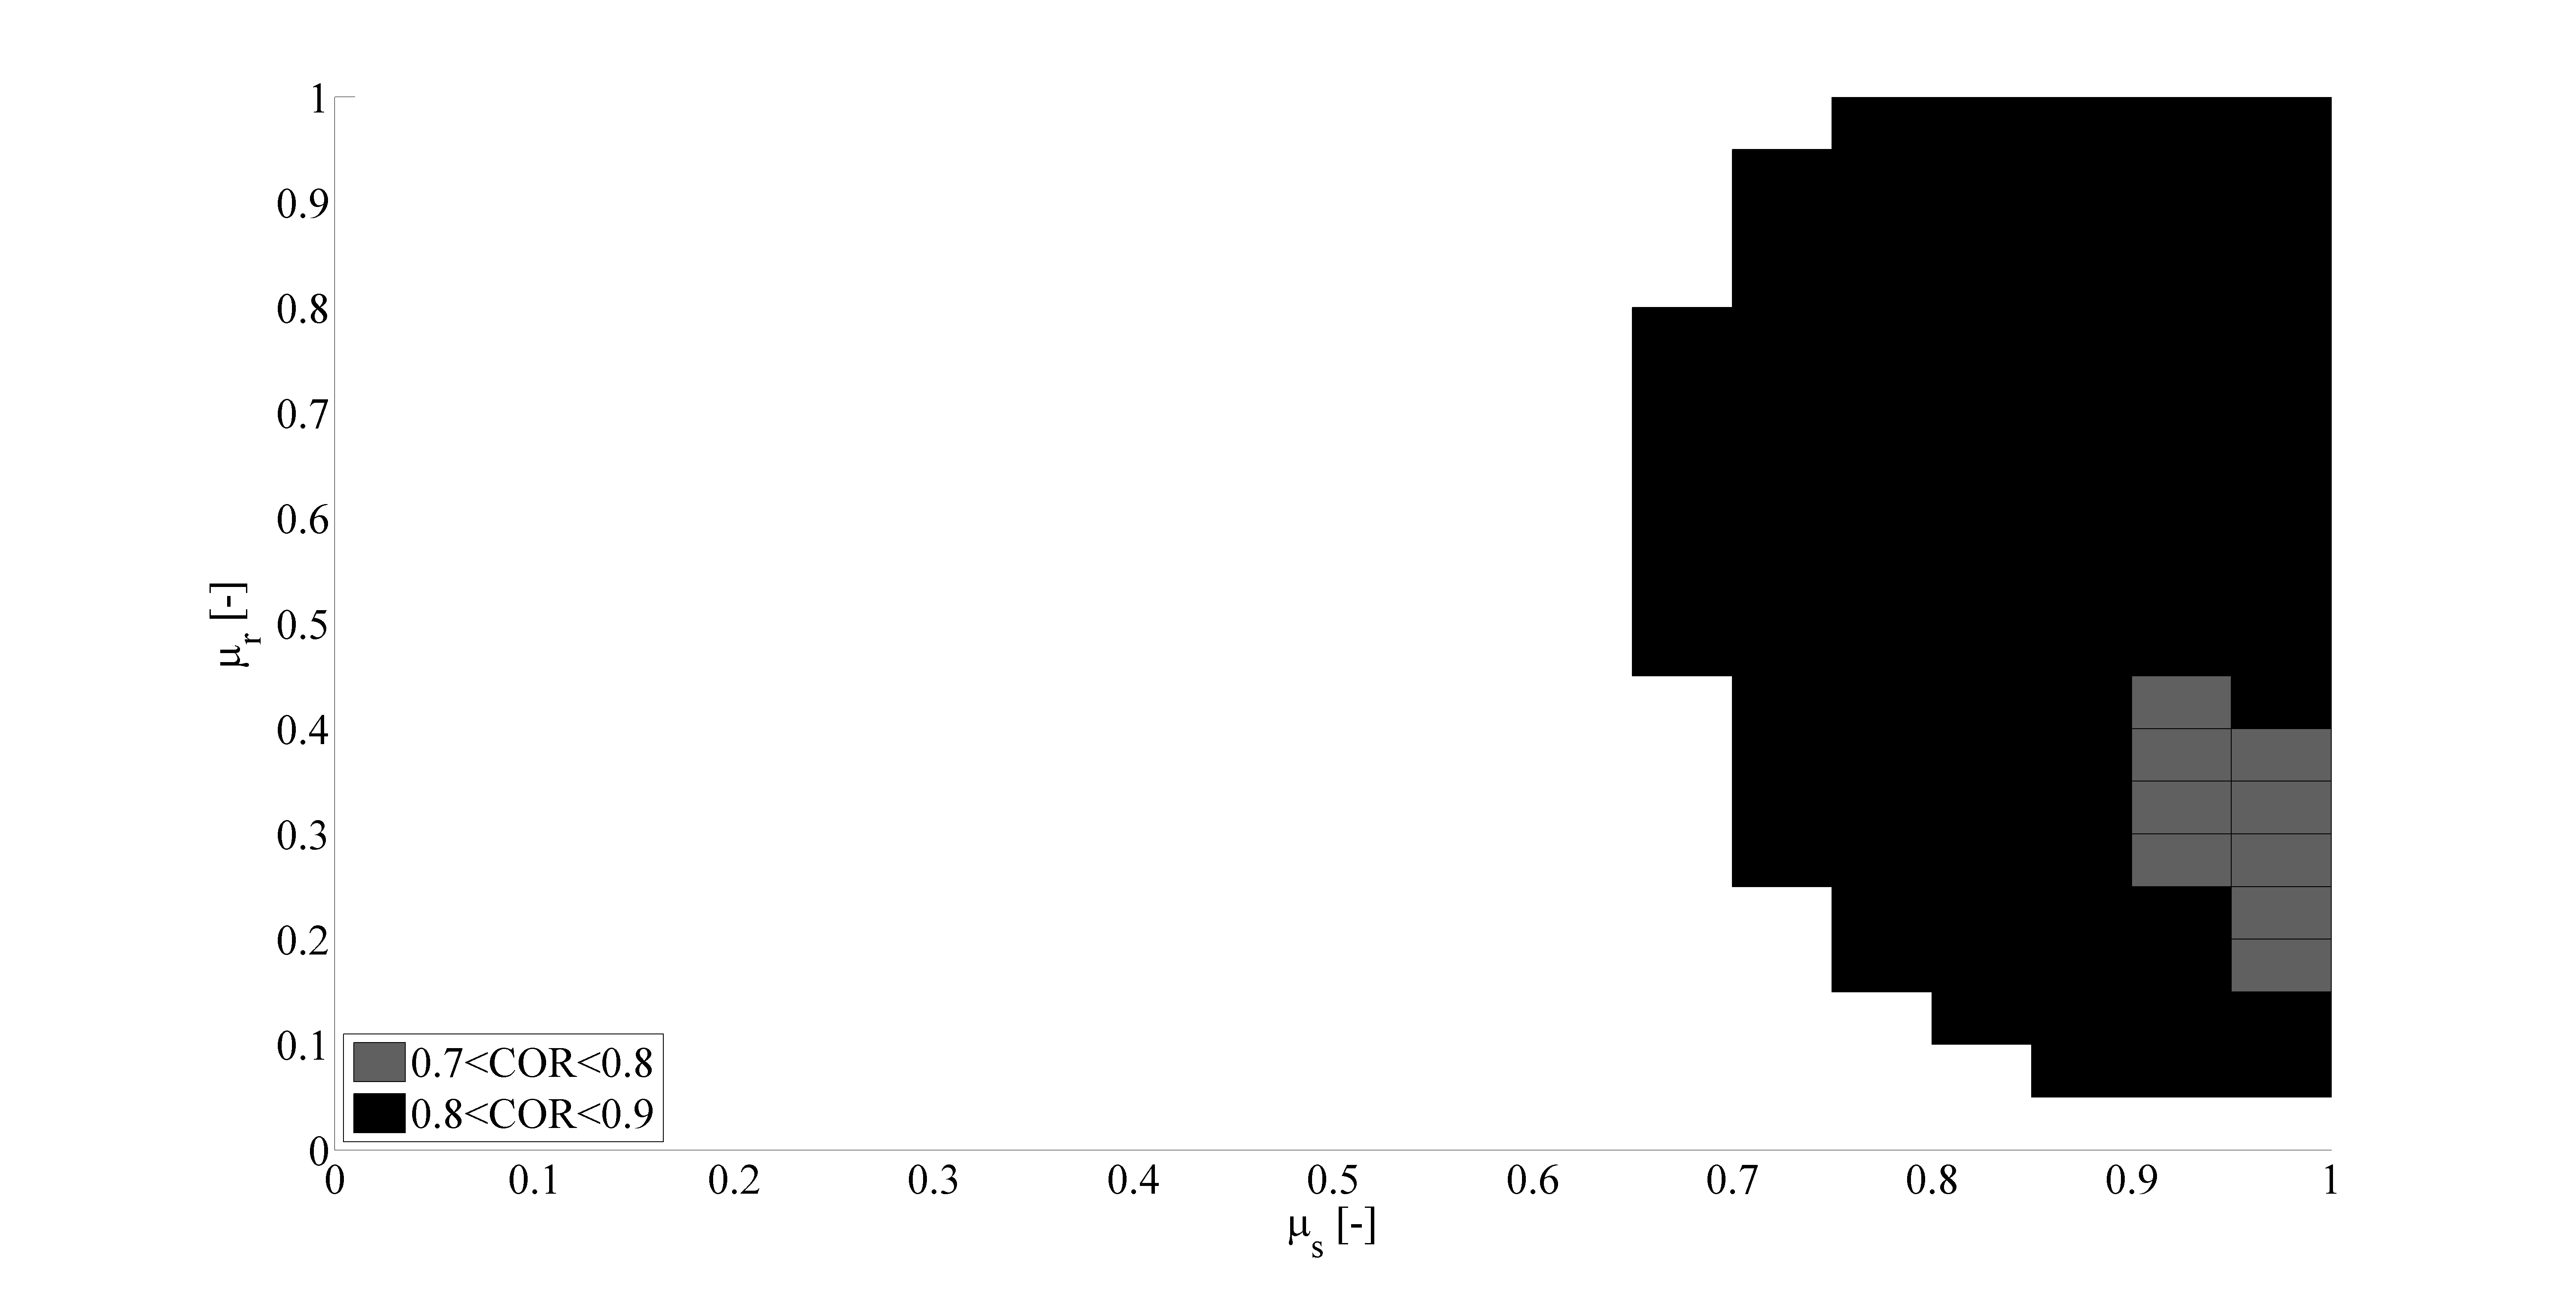
\includegraphics[width=.48\columnwidth]{images/030cloudpirker12schulze10070}
	  \label{fig:030cloudpirker12schulze10070}
  }
  \\
  \caption{Density plot comparison of SCT results.}
  \label{fig:080sctdensityplots}
\end{figure}
\begin{figure}[htbp]
\centering 
  \subfloat[Parameter space plot, $AoR_{exp} = 38.85 ^\circ$.]{
	  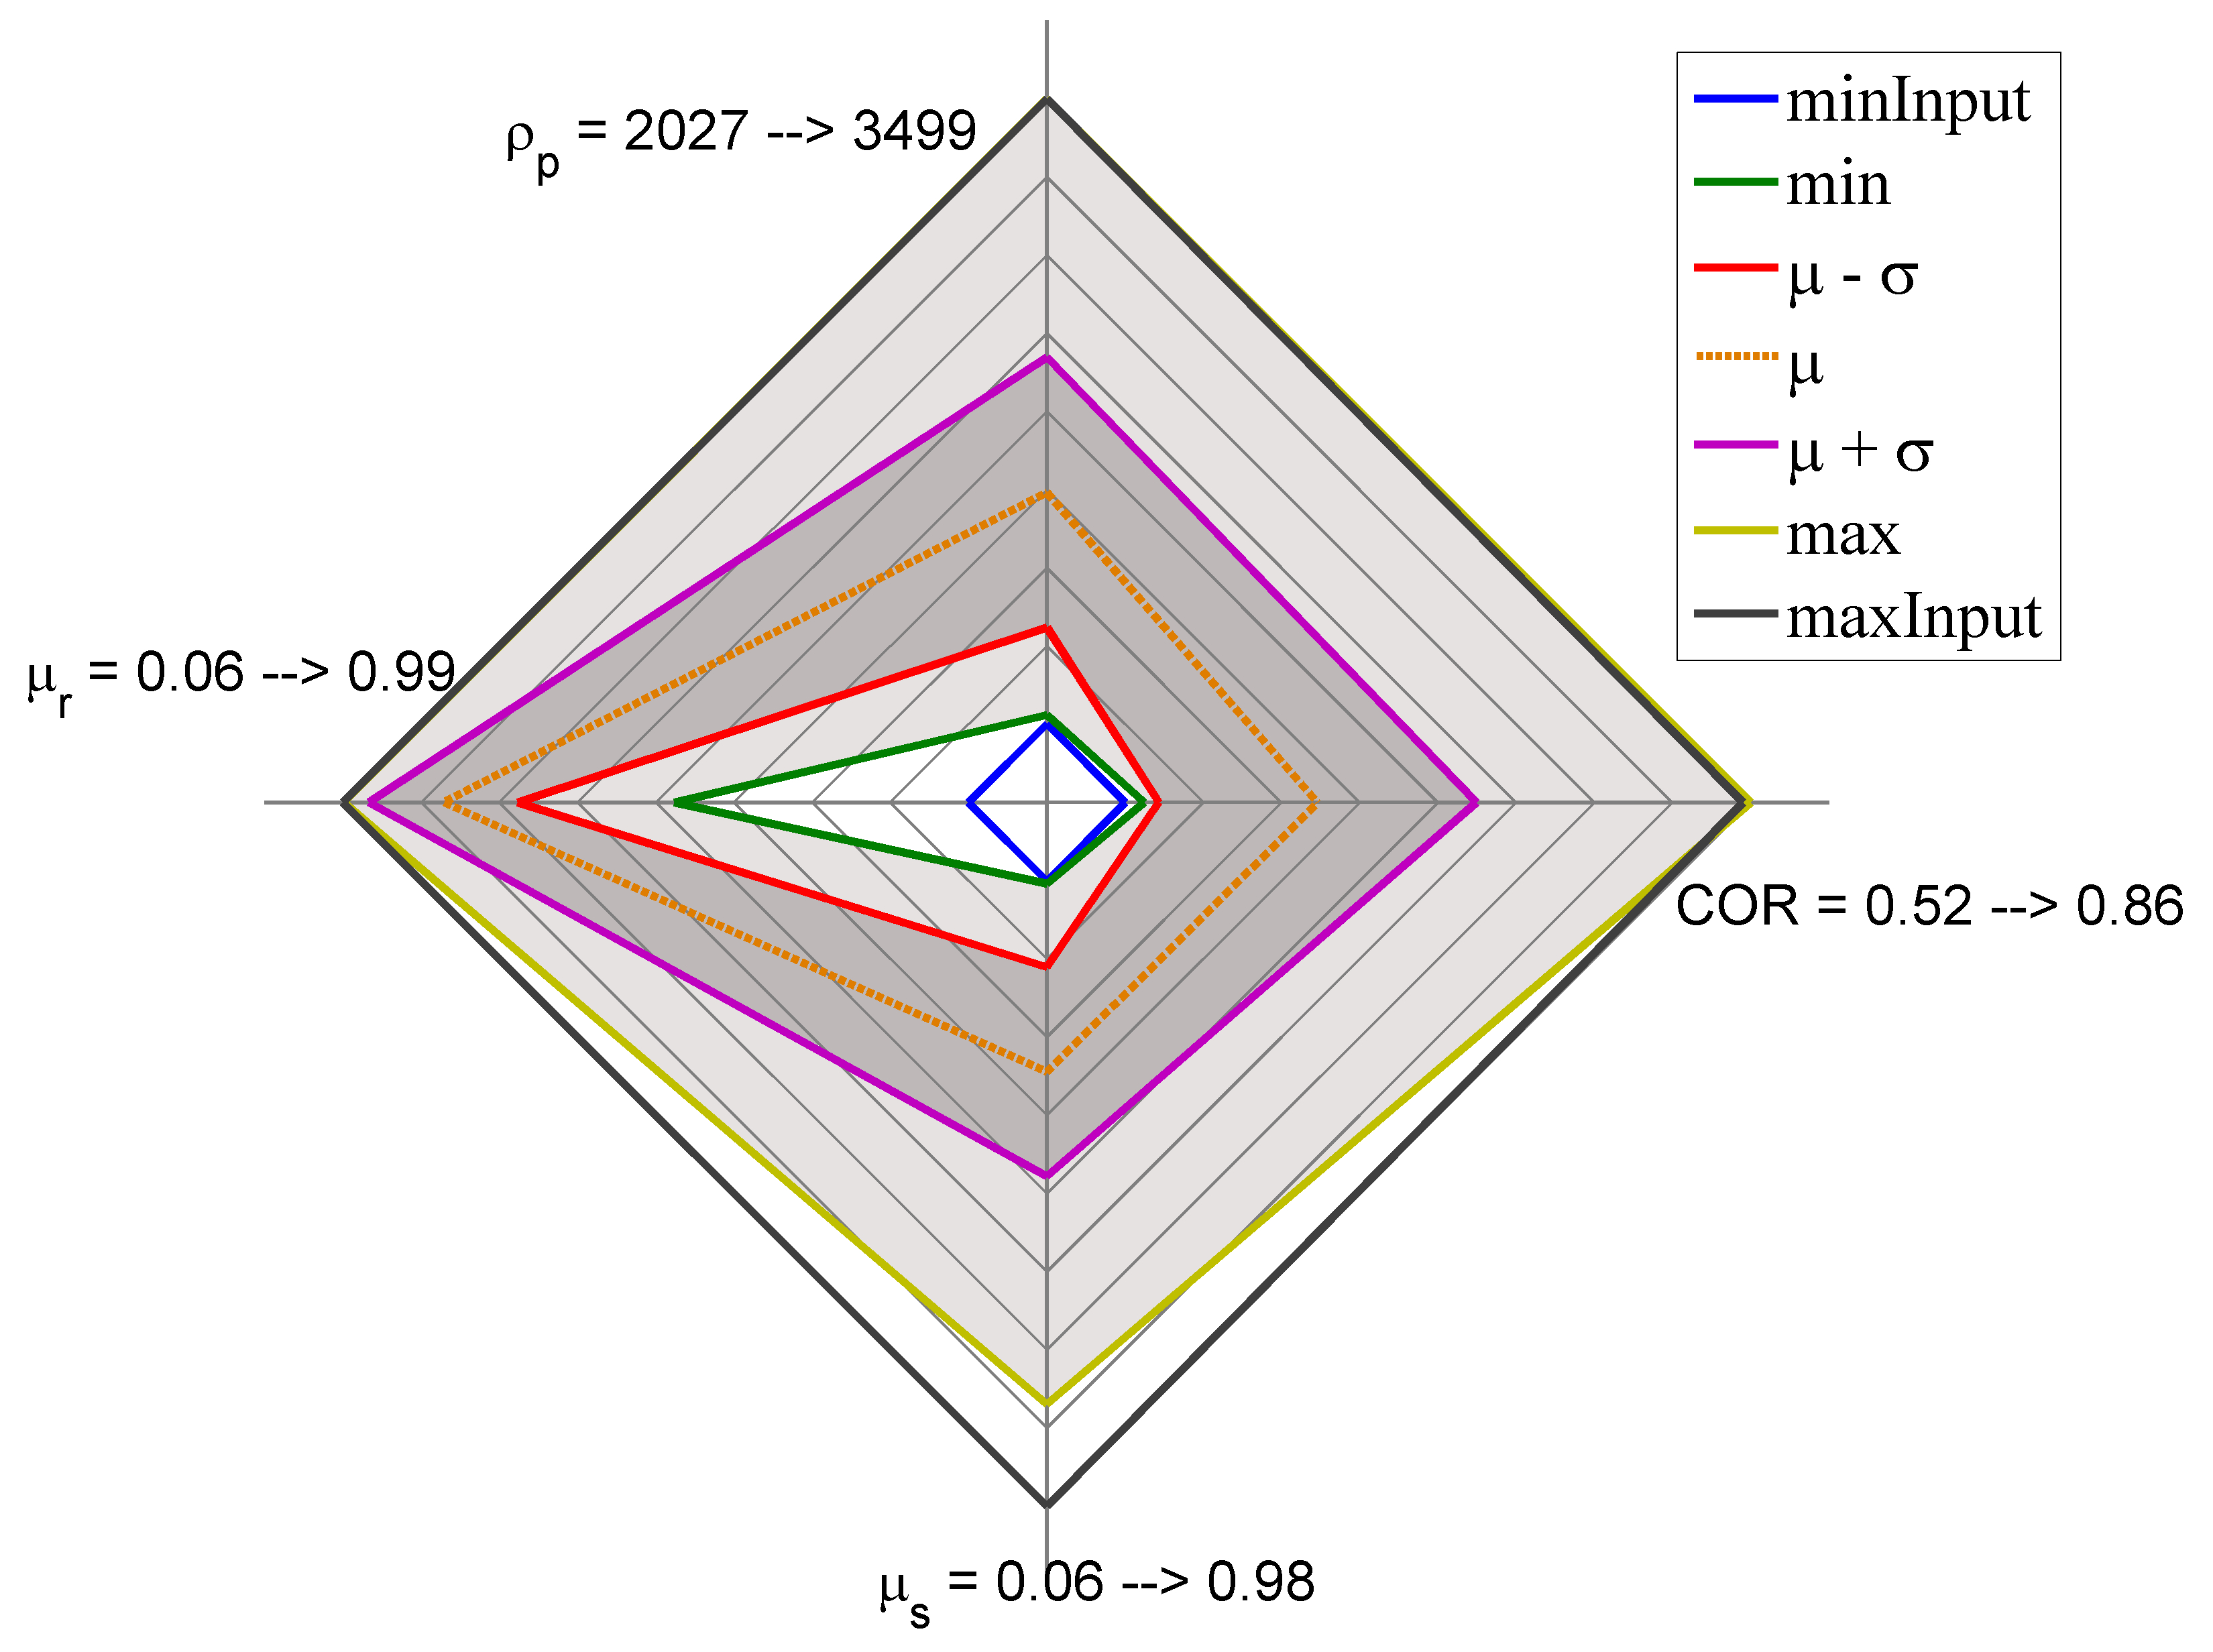
\includegraphics[width=.40\columnwidth]{images/031radarpirker1aor}
	  \label{fig:031radarpirker1aor}
  }
  \quad
    \subfloat[Box plot, $AoR_{exp} = 38.85 ^\circ$.]{
	  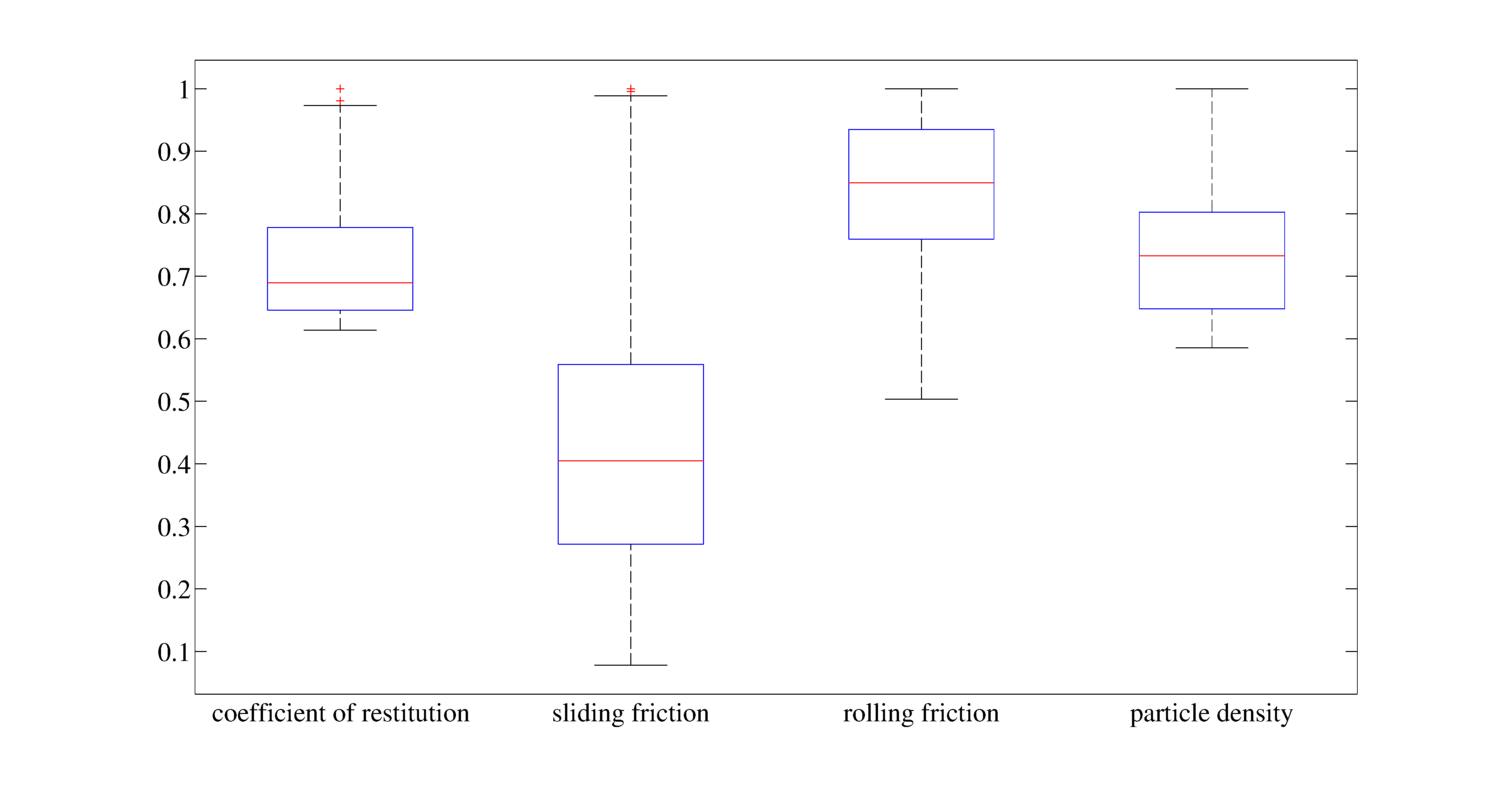
\includegraphics[width=.40\columnwidth]{images/076aorboxplot}
	  \label{fig:076aorboxplot}
  }
  \\
  \subfloat[Parameter space plot, $AoR_{exp} = 38.85 
        ^\circ$ \& $SSC$: $\sigma_n=10070$ Pa.]{
	  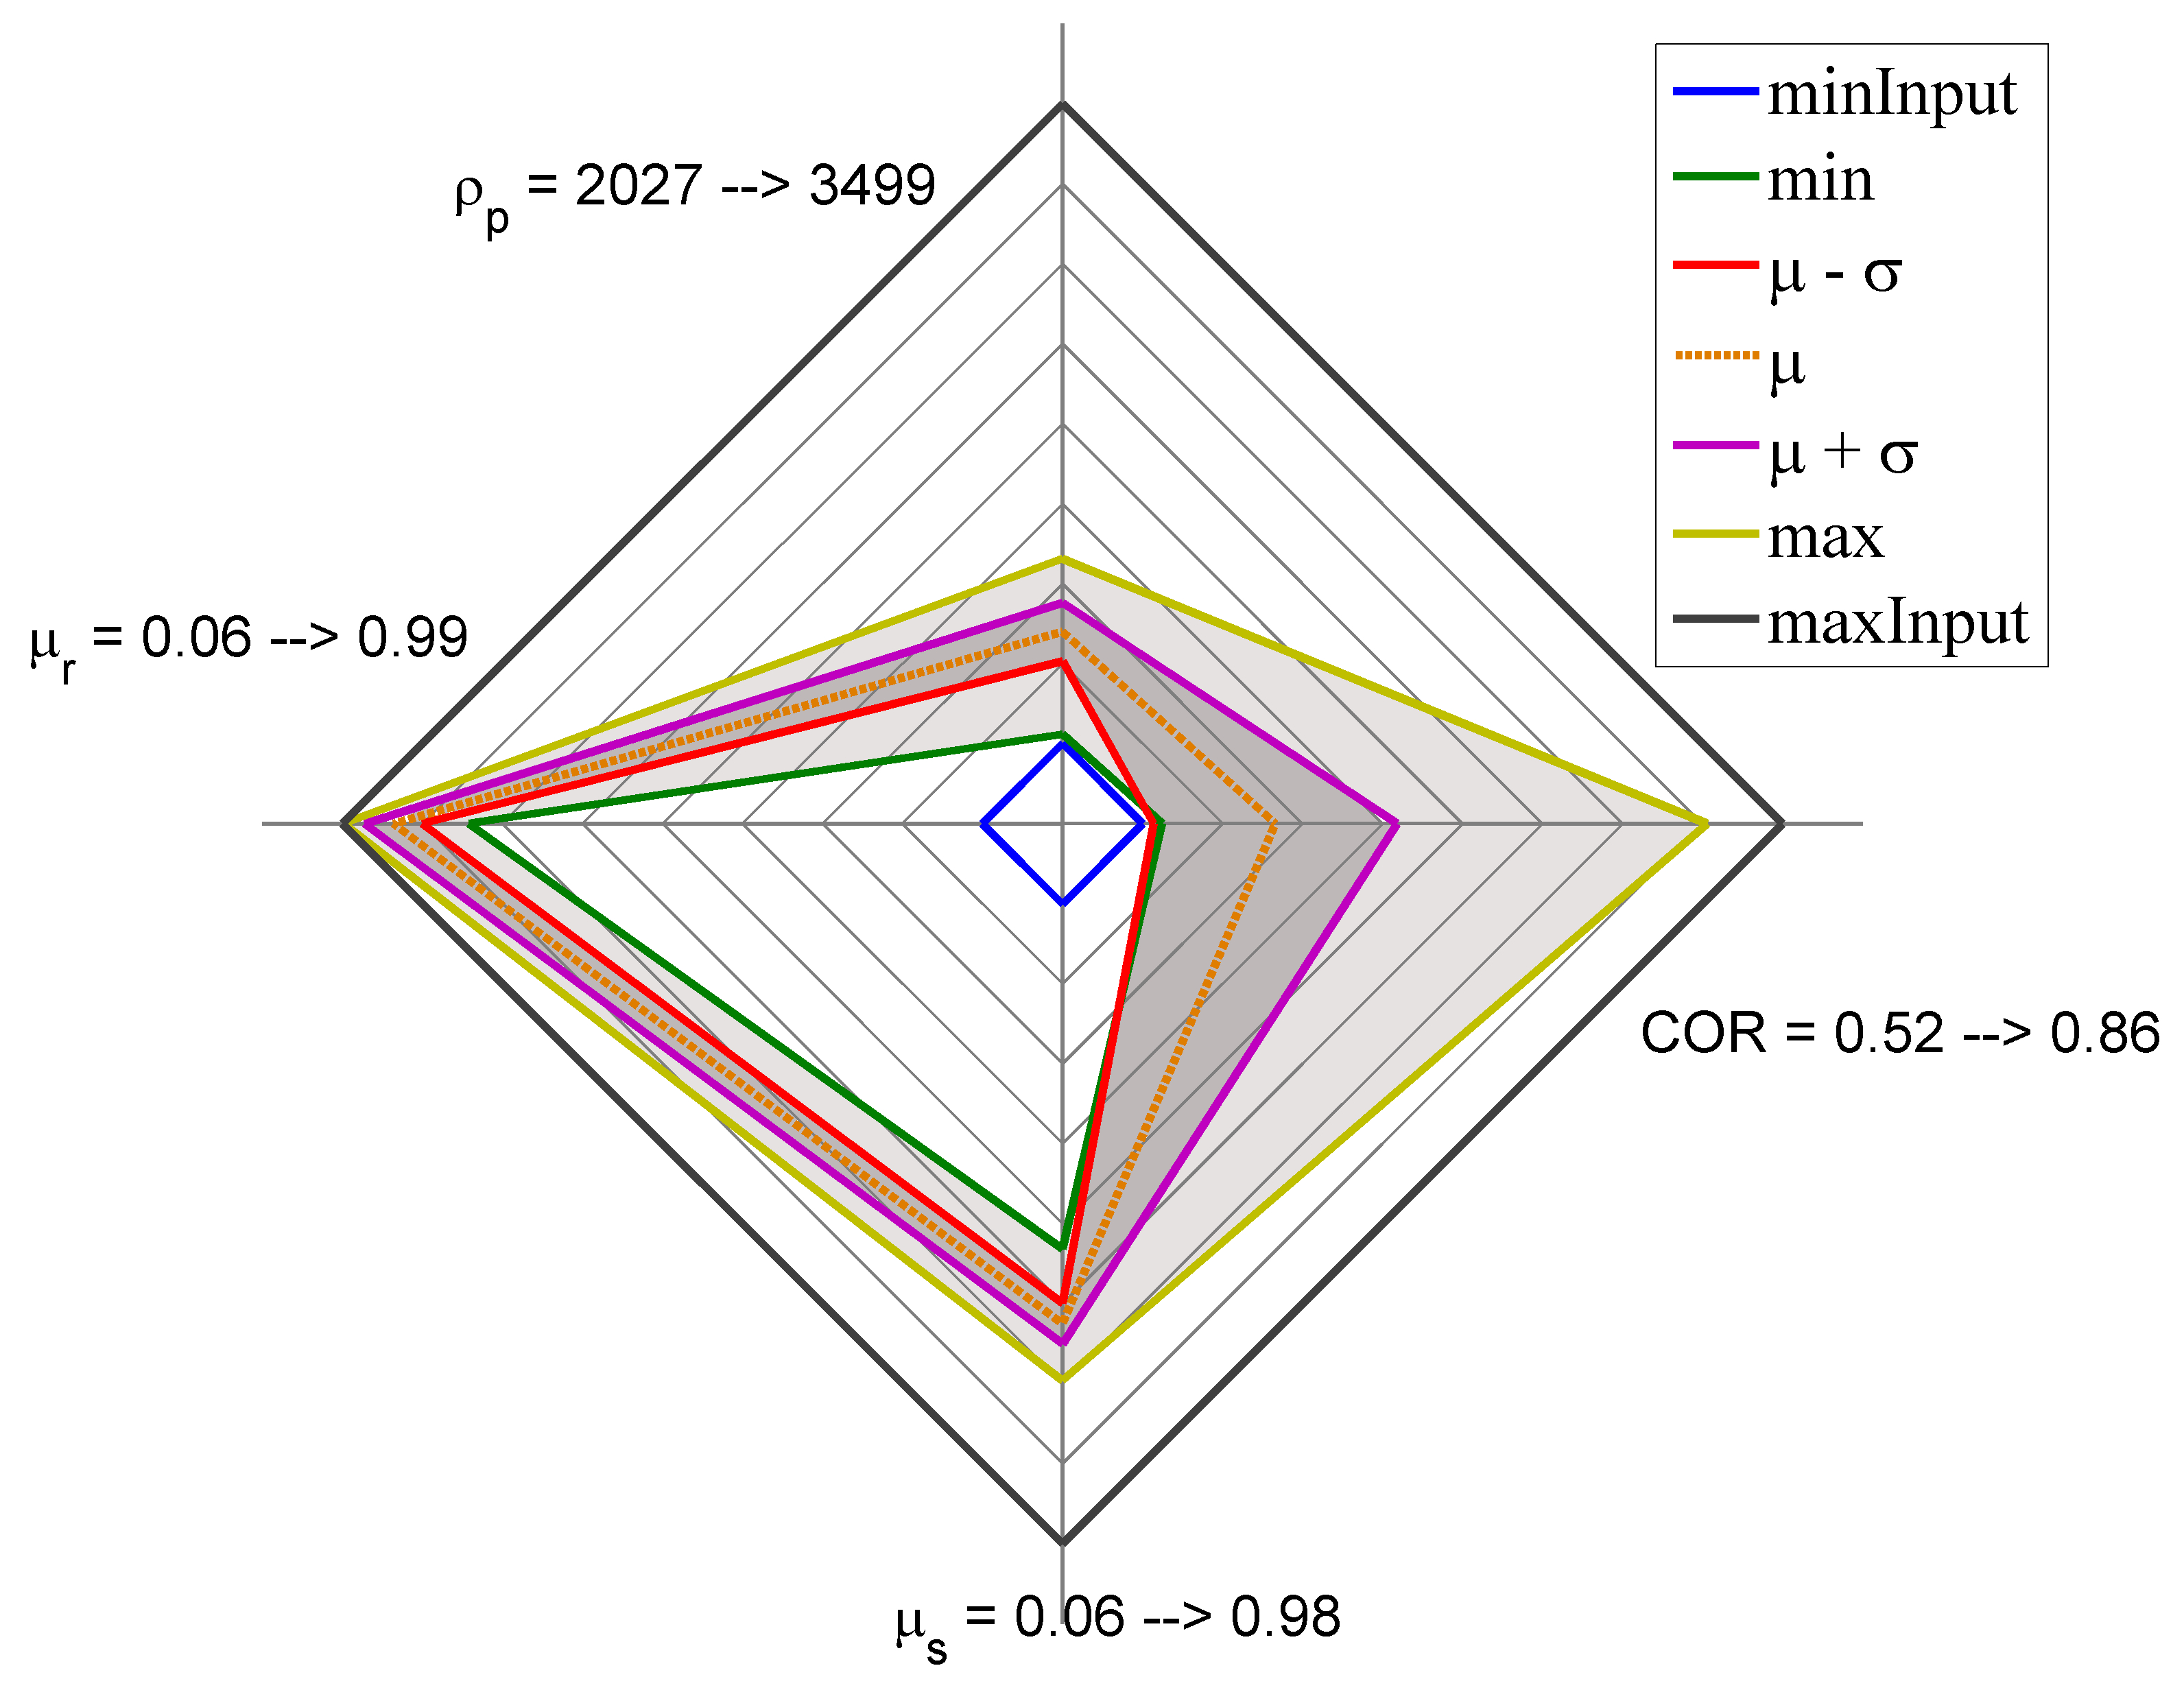
\includegraphics[width=.40\columnwidth]{images/033radarpirker1schulze10070aor}
	  \label{fig:033radarpirker1schulze10070aor}
  }
  \quad
    \subfloat[Box plot, $AoR_{exp} = 38.85
        ^\circ$ \& $SSC$: $\sigma_n=10070$ Pa.]{
	  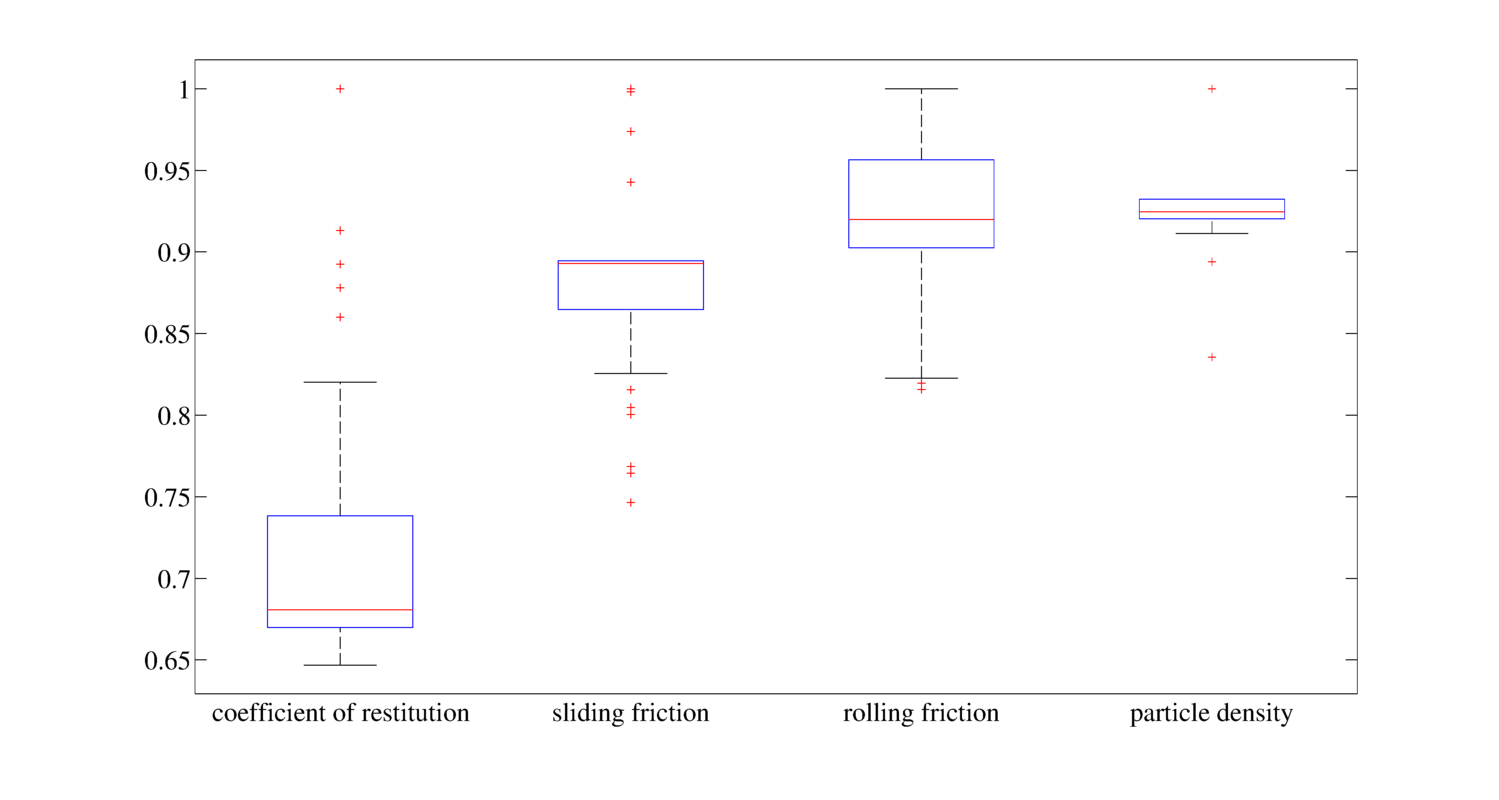
\includegraphics[width=.40\columnwidth]{images/078mergeboxplot}
	  \label{fig:078mergeboxplot}  }
  \\
  \caption{AoR and merge parameter space plots.}
  \label{fig:081aorandmergeparameterspaceplots}
\end{figure}
